\documentclass[12pt,openany]{book}
\usepackage{lmodern}
\usepackage{setspace}
\setstretch{1.25}
\usepackage{amssymb,amsmath}
\usepackage{ifxetex,ifluatex}
\usepackage{fixltx2e} % provides \textsubscript
\ifnum 0\ifxetex 1\fi\ifluatex 1\fi=0 % if pdftex
  \usepackage[T1]{fontenc}
  \usepackage[utf8]{inputenc}
\else % if luatex or xelatex
  \ifxetex
    \usepackage{mathspec}
  \else
    \usepackage{fontspec}
  \fi
  \defaultfontfeatures{Ligatures=TeX,Scale=MatchLowercase}
\fi
% use upquote if available, for straight quotes in verbatim environments
\IfFileExists{upquote.sty}{\usepackage{upquote}}{}
% use microtype if available
\IfFileExists{microtype.sty}{%
\usepackage{microtype}
\UseMicrotypeSet[protrusion]{basicmath} % disable protrusion for tt fonts
}{}
\usepackage[left=4cm, right=3cm, top=3cm, bottom=3cm]{geometry}
\usepackage[unicode=true]{hyperref}
\hypersetup{
            pdfborder={0 0 0},
            breaklinks=true}
\urlstyle{same}  % don't use monospace font for urls
\usepackage{longtable,booktabs}
\usepackage{graphicx,grffile}
\makeatletter
\def\maxwidth{\ifdim\Gin@nat@width>\linewidth\linewidth\else\Gin@nat@width\fi}
\def\maxheight{\ifdim\Gin@nat@height>\textheight\textheight\else\Gin@nat@height\fi}
\makeatother
% Scale images if necessary, so that they will not overflow the page
% margins by default, and it is still possible to overwrite the defaults
% using explicit options in \includegraphics[width, height, ...]{}
\setkeys{Gin}{width=\maxwidth,height=\maxheight,keepaspectratio}
\IfFileExists{parskip.sty}{%
\usepackage{parskip}
}{% else
\setlength{\parindent}{0pt}
\setlength{\parskip}{6pt plus 2pt minus 1pt}
}
\setlength{\emergencystretch}{3em}  % prevent overfull lines
\providecommand{\tightlist}{%
  \setlength{\itemsep}{0pt}\setlength{\parskip}{0pt}}
\setcounter{secnumdepth}{5}
\usepackage[none]{hyphenat}
\usepackage[cmyk]{xcolor} % Recommended by US-AB
\usepackage{lmodern} % Recommended by US-AB
\usepackage{fancyhdr}
\usepackage{etoolbox}
\patchcmd{\chapter}{\thispagestyle{plain}}{\thispagestyle{fancy}}{}{} % Removes plain pagestyle from chapter headings (otherwise, page numbers are centered)
\AtBeginDocument{\addtocontents{toc}{\protect\thispagestyle{empty}}} 
\pagestyle{empty} % This makes ToC without header/footer
\usepackage[skip=15pt]{caption} % This should increase space below captions (not tested)
\raggedbottom
\usepackage[noindentafter]{titlesec}
\usepackage{titlesec}
\titleformat{\chapter}{\normalfont\bfseries}{\thechapter.}{15pt}{}\titlespacing*{\chapter}{0pt}{-50pt}{0pt}
\titleformat{\section}{\normalfont\bfseries}{\thesection.}{1em}{}\titlespacing*{\section}{0pt}{0pt}{0pt}
\titleformat{\subsection}[runin]{\normalfont\bfseries}{\thesubsection.}{1em}{}

\usepackage{CJKutf8} % For Mandarin in Acknowledgments

% For guiding quote in beginning of intro:
\makeatletter
% \renewcommand{\@chapapp}{}% Not necessary...
\newenvironment{chapquote}[2][2em]
  {\setlength{\@tempdima}{#1}%
   \def\chapquote@author{#2}%
   \parshape 1 \@tempdima \dimexpr\textwidth-2\@tempdima\relax%
   \itshape}
  {\par\normalfont\hfill--\ \chapquote@author\hspace*{\@tempdima}\par\bigskip}
\makeatother
\usepackage{placeins}
\usepackage{titlesec}
\newcommand{\sectionbreak}{\clearpage}
\usepackage{amsmath}
\usepackage{wrapfig}
\usepackage{caption}
\captionsetup[figure]{font=scriptsize}
\usepackage{float}
\usepackage{amssymb}

\author{}
\date{\vspace{-2.5em}}

\begin{document}

{
\setcounter{tocdepth}{3}
\tableofcontents
}
\cleardoublepage
\pagestyle{fancy} \fancyhf{} \renewcommand{\headrulewidth}{0pt}
\fancyfoot[LE,RO]{\thepage} \renewcommand{\floatpagefraction}{.9}
\setcounter{page}{9}

\chapter*{Abbreviations}\label{abbreviations}
\addcontentsline{toc}{chapter}{Abbreviations}

\begin{tabular}{ll}
\toprule
Abbreviation & Term\\
\midrule
RPF & Ribosome Protected Fragment\\
TOP & Terminal oligopyrimidine\\
TE & Translation Efficiency\\
UTR & Untranslated region\\
uORF & upstream open reading frame\\
\bottomrule
\end{tabular}

\chapter{Introduction}

\section{Gene expression}\subsection{The central dogma of gene expression}

The whole genetic code of an organisms i stored as deoxyribonucleic acid
(DNA) molecules in a double stranded formation as chromosomes.
Chromosomes hold the DNA in a condensed state using chromatin, a complex
of DNA and proteins, structures. For transcription of DNA to occur
chromatin is remodeled to expose promotor regions in the DNA to which
fators assisting in transcription bind. One of these factors is DNA
polymerase that unravels the double-stranded DNA and creates a
single-stranded copy called ribonucleic acid (RNA) transcripts. This
copy is less stable due to its single strandedness and therefore only
temporary. The RNA transcripts undergo processing by which multiple
different transcript varaints coming from the same genomic region can be
produced. The protein coding portion of these transcripts are called
mRNAs. Once formed mRNAs are transported into the cytoplasm where they
are either degraded or associate with ribosomes. These ribosomes
translate the mRNAs into proteins by which the genetic information then
is expressed. Synthesised proteins, if no longer needed in the cell, can
be degraded by proteosomes (\textbf{see figure \ref{fig:geneExprPath}}).
This flow of genetic information into expressed proteins is commonly
referred to as the central dogma in molecular biology (Crick, 1970).
\clearpage

\begin{figure}
  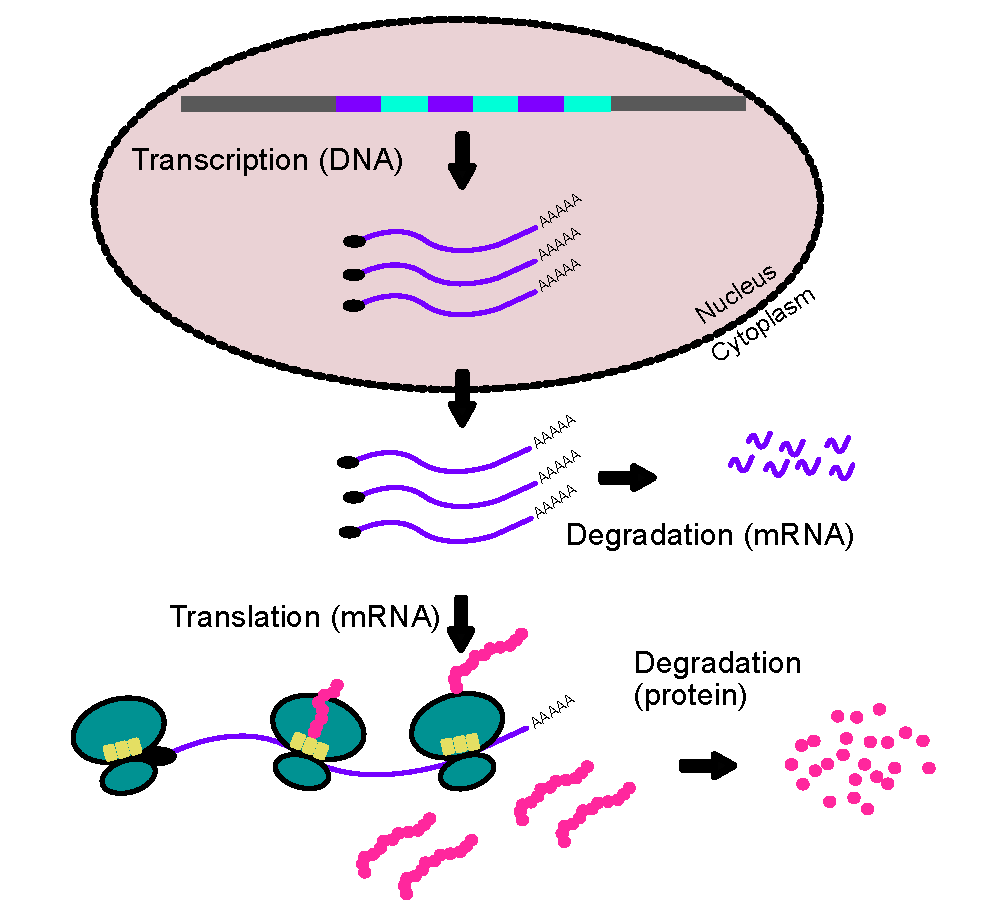
\includegraphics{./figures/geneExprPath_2.pdf}
  \caption{The gene expression pathway - DNA is transcribed in pre-mRNA containing a 5' cap (black oval) introns (teal boxes),exons (purple boxes) and a poly(A) tail. RNAs are processed into mRNAs consisting out ouf a 5' cap,exons and a poly(A) tail is then transported out of the cellular nucleus into the cytoplasm. Within the cytosplasm mRNAs can be degradated or translated  into proteins depending on cellular demands. Synthesised proteins can be degraded by proteosomes. \label{fig:geneExprPath}}
\end{figure}

\clearpage
\subsection{Contribution to gene expression} Proteins are the last
product of the gene expression pathway and carry out the vast majority
of all cellular functions. While it is apparent that modulation of
protein levels will offer information on the changes in gene expression,
it cannot completely answer the question as to why the levels change. In
a disease context, protein levels alone might offer sufficient insight
to explain phenotypic differences. However, how these differences arise
machanistically, which often poses as target for therapeutic strategies
in cancer, is obscured.

Experimental methods to measure gene expression at different steps are
often to referred as ``omics'' (i.e.~proteomics for protein expression,
transcriptomics for mRNA expression). These methods provide snapshots of
the step under scrutiny in a specific context (steady state or
perturbation) for a large portion of genes or proteins. Transcriptomics
studies approach gene expression with the assumption that mRNA
expression results in protein expression changes and can therefore be
used as a proxy for them. However, this view got challanged by landmark
studies that observed a poor mRNA to protein correlation and indicated a
larger role of post transcriptional regulation in gene expression that
previously assumed (J. Lu, Tomfohr, \& Kepler, 2005,Vogel \& Marcotte
(2012),de Sousa Abreu, Penalva, Marcotte, \& Vogel (2009),Schwanhäusser
et al. (2011),Silva \& Vogel (2016)).

The debate on which step of the gene expression pathway contributes most
is ongoing, nevertheless an understanding has been reached that the
cellular context at is a major determinant. At steady state mRNA levels
seem to explain protein abundance best, however in perturbed systems the
contribution of transcript abundance is shifted away to other steps (Y.
Liu, Beyer, \& Aebersold, 2016). For example in a study that challanged
immune cells, protein levels were dependent on cellular transcript
levels (Jovanovic et al., 2015). In contrast a study investigating cells
under stress observed extensive modulation at the protein levels,
whereas mRNA transcript abundance was only mildly affected (Cheng et
al., 2016).

While the contribution of different steps of the gene expression is
dependent on many different factors, e.g.~cellular state, treatments,
mRNA translation (synthesis of proteins) is an essential process of this
pathway. Furthermore, dysregulation of mRNA translation has been
observed in a plethora of diseases, ranging from neurological disorders
to cancer({\textbf{???}},Ruggero (2013)). This thesis will focus on the
role of mRNA translation in the context of cancer. \clearpage

\section{mRNA translation}

mRNA translation is the most energy demanding process in the cell and is
therefore tightly linked to the energy metabolism (Buttgereit \& Brand,
1995). Translation plays major roles in cellular functions such as
prolifertion (increase cell count) and growth (expand cell size) and
deregulation thereof is often found in cancer (\textbf{see section
\ref{translationInCancer}}) but also associated with other diseases
(Graff et al., 2009,I. Topisirovic \& Sonenberg (2011),Lee et al.
(2021)). To make inferences on differences in mRNA translation we
capture the transcriptome available in the cytoplasm as well as the
portion of mRNAs that is actively translated. This enables us to
interrogate two prominent players of gene expression at once.

\subsection{overview of an mRNA}

After transcription primary RNA transcripts are processed into mRNAs
which is the products that will be translation. The coding region of an
mRNA is flanked by untranslated region that exert translational control
over the mRNA (see \ref{UTR}). The 5' has a cap that is important for
mRNA translation initiation(Grifo, Tahara, Morgan, Shatkin, \& Merrick,
1983), while the 3' end has a poly-A tail protecting the mRNA against
degradation (Wilusz, Wormington, \& Peltz, 2001). Multiple different
mRNAs (isoforms or transcript variants) from the same genomic region
exist. These variants arise due to a process called alternative splicing
which alters the exon composition (i.e.~coding region) of an mRNA with
distinct functions or properties (Joly Anne-Laure et al., 2018).

\begin{wrapfigure}{o}{1\textwidth}
  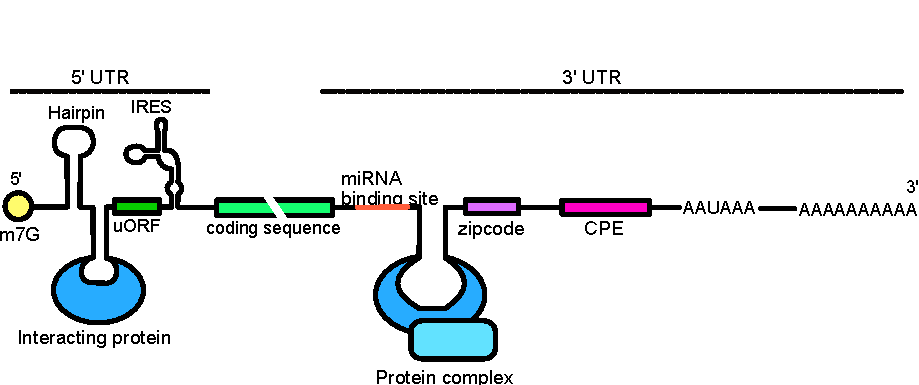
\includegraphics{./figures/UTRFeatures.pdf}
  \caption{ An mRNA consists of a coding sequence (green), 5' (light orange) and 3' (purple) untranslated regions flanking the coding sequence, a 5' cap and a poly-A tail. Located within the 5' and 3' untranslated region are cis elements (light red boxes) that can exert translational control by interfering with ribosomal movement along the mRNA or interact with trans factors (blue and red) or recruit the 43s ribsome (dark green) to the mRNA (see section \ref{UTR}). The codon composition of the coding sequence also influences translation (see section \ref{tRNA}).   
 \label{fig:UTRFeat}}
\end{wrapfigure}

\clearpage
 For the vast majority of protein coding mRNAs, eukaryotic mRNA
translation occurs in the cytoplasm, however a small subset of mRNAs is
translated in the mitochondria. mRNA translation is a process that
includes initiation, elongation, termination and ribosome recycling and
is an essential process \textbf{see Figure \ref{fig:doodlemRNASteps}}.
During the initiation phase a ribome will associate with the mRNA and
starts scanning along the mRNA for a start codon to begin synthesis of
the polypeptide chain by incorporating amino acids. The order by which
amino acids are incorporated are dictated by subsequent codons of the
open reading frame (ORF). Redundancy in the codon availability allows
that amino acids have multiple assigned codons, for example lysine is
encoded by AAA and AAG. Amino acids are transferred to the ribosome by
specialised RNAs called transfer RNAs (tRNA) that can recognise the
genetic code in the mRNA. The availability of tRNAs as well as their
modification can influence the rate of elongation (see \ref{tRNA}) Once
the ribosome encounters a stop codon translation will terminate and the
polypeptide chain will be released. The ribosome then disassociates from
the mRNA and the ribosome can be recycled to engage translation of the
same or another mRNA. The following setions describe these processes in
more detail.

\begin{wrapfigure}{o}{1\textwidth}
  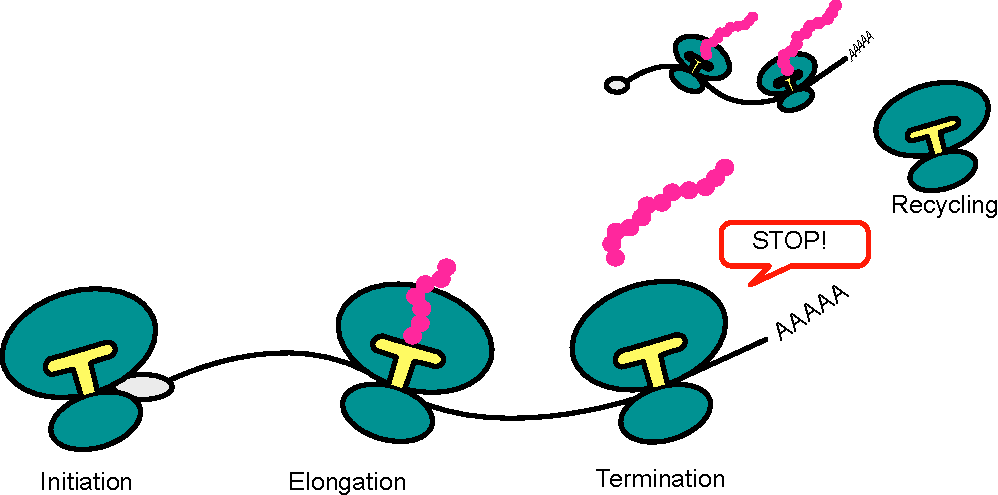
\includegraphics{./figures/doodleTranslation.pdf}
  \caption{mRNA translation initiation, elongation, termination and ribosome recycling steps - The ribosome binds to the mRNA and initiates scanning for a start codon. The elongation phase incorporates amino acids into a polypeptide chain (i.e. the protein product). Once the end of the coding sequence is detected, by recognition of stop codons, the ribosome terminates translation and releases the polypeptide chain. The ribosome can then be recycled to participate in the translation of another mRNA or reinitiate. \label{fig:doodlemRNASteps}}
\end{wrapfigure}

\clearpage

\subsection{initiation} \label{initiation}

For the initiation to commence, in eukaryotes, two complexes are
required; the pre-initiation complex (PIC) and the eukaryotic initiation
factor 4F (eIF4F) complex. Both these complexes are governed by
signalling pathways that regulate their availability dependent on
cellular cues. The PIC consists of the methionyl-initiatior transfer RNA
(met-tRNAi) in a ternary complex (TC) with guanosine triphosphate (GTP)
bound eIF2 (Asano, Clayton, Shalev, \& Hinnebusch, 2000). eIF4F is the
translation initation complex containing three EIFs; eIF4E, the 5' cap
binding protein, eIF4G a scaffold protein and eIF4A and RNA helicase
(Grifo et al., 1983,Hinnebusch (2006)). eIF4F recruites the PIC to the
5' cap of the mRNA after which scanning for a start codon (AUG) occurs.
After AUG recognition eIF2-GTP is hydrolyzed forming a stable 48S PIC.
Afterrelease of eIF2-GTP the 60S ribosomal subunit joins to form the 80S
ribosome and protein synthesis can commence (\textbf{Figure
\ref{initiation}}).

\begin{wrapfigure}{o}{.6\textwidth}
  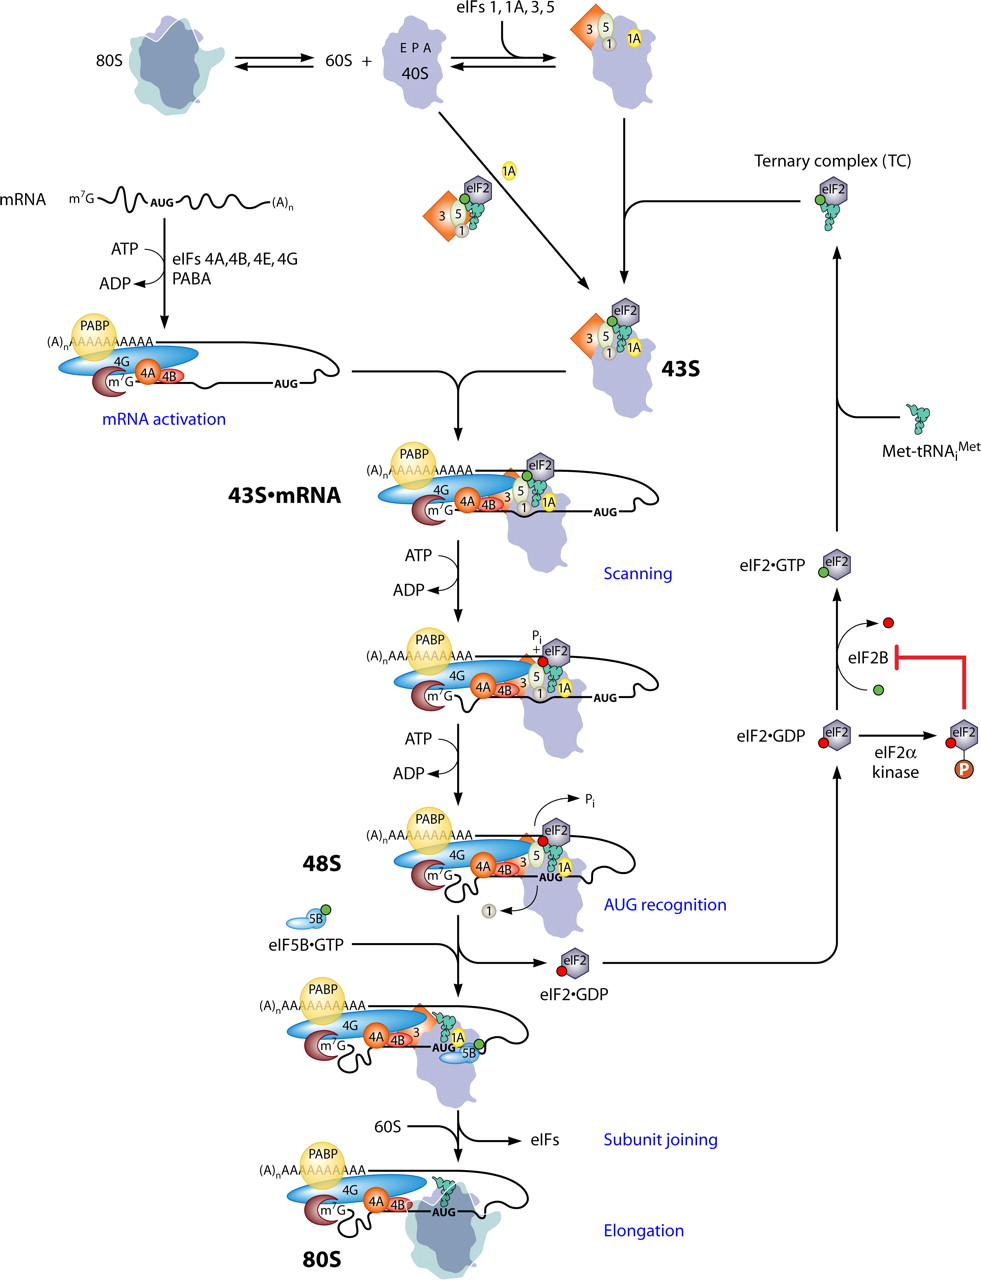
\includegraphics{./figures/initiation.jpg}
  \caption{Pathway of eukaryotic translation initiation via ribosomal scanning.
 \label{fig:initiation}}
\end{wrapfigure}

\subsection{elongation}

The 80S ribosome contains three sites important for decoding an mRNA;
the acceptor (A), peptidyl (P) and Exit (E) sites. During elongation in
eukaryotes animoacytelated tRNAs are delivered to the A-site in a
ternary complex with eukaryotic elongation factor 1A (eEF1A). When the
tRNA recognises its cognate codon and pairs, a bond between the amino
acid and the polypeptide chain is formed. The formation of the bonds
causes the ribosomal units to rotate in relation to each other (Munro,
Altman, O'Connor, \& Blanchard, 2007,Moazed \& Noller (1989)). The
rotation causes a shift of the tRNA acceptor ends from the A and P to
the P and E sites, wheras the codon end remains in the A and P site.
This is the ``hyrbid'' state of the tRNAs in the ribosome(Dorner,
Brunelle, Sharma, \& Green, 2006). eEF2 then promotes the translocation
by which the codon ends of the tRNA follow into the P and E sites. The
deacytelated tRNA is then released from the ribosome. This process is
repeated until a stop codon (UAA, UGA or UAG) is detected by the
ribosome which terminates translation.

\begin{wrapfigure}{o}{.6\textwidth}
  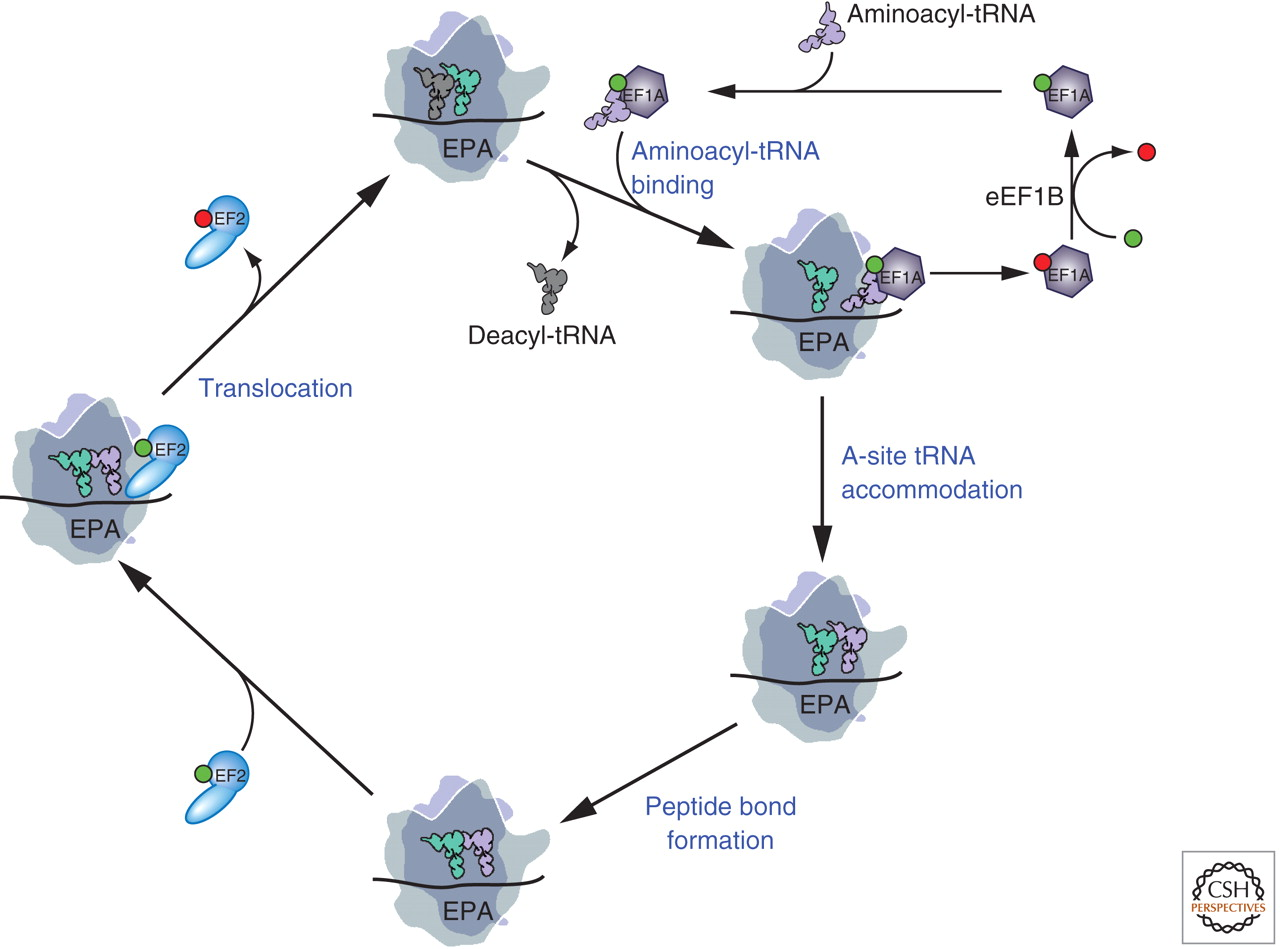
\includegraphics{./figures/elongation.jpg}
  \caption{Model of the eukaryotic translation elongation pathway.Thomas E. Dever, and Rachel Green Cold Spring Harb Perspect Biol 2012;4:a013706. Reprinted with permission. ©2012 by Cold Spring Harbor Laboratory Press
 \label{fig:elongation}}
\end{wrapfigure}

\clearpage

\subsection{termination and recycling}

mRNa translation termination is facilitated by two release factors
(eRF), eRF2 and eRF3-GTP(I. Stansfield et al., 1995,Alkalaeva, Pisarev,
Frolova, Kisselev, \& Pestova (2006)). A TC containing eRF2 and eRF3-GTP
binds to the A-site of the ribosome upon recognition of a stop codon.
This causes an ATP hydrolysis event resulting in a conformational change
and release of the polypeptide chain. eRF1 and the ATP binding cassette
protein (ABCE1) together promote the splitting of the 60S and 40S
subunits after which they can be recycled(Pisarev et al., 2010,Dever \&
Green (2012),Hellen (2018)).

\subsection{Translation efficiency}

Each ribosome synthesises a single protein during translation of an mRNA
from start to end. Typically an mRNA is loaded with multiple ribosomes
(i.e.~polysomes). Therefore, the rate at which proteins can be
synthesised is dependent on the availability of mRNAs as well as
ribosome dynamics at the initiation, elongation and termination of mRNA
translation.

\section{Regulation of mRNA translation}

Of the heretofore presented steps of mRNA translation the initiation is
the most regulated step. From the perspective that mRNA translation
contributes most to the cellular energy consumption, of which the
initiation requires ATP, this process ought to be strictly regulated
(Buttgereit \& Brand, 1995,Jackson (1991),N. Sonenberg \& Hinnebusch
(2009)). Nevertheless, translation can also be regulated at the
elongation (Richter \& Coller, 2015) and termination(Dever \& Green,
2012) phases albeit to a lesser extent. Dynamic modulation of mRNA
translation can be achieved through signalling pathways as well as
several distinct cis and trans elements in both untranslated regions
(UTRs) of an mRNA (\textbf{Figure \ref{fig:UTRFeat}}).

\subsection{Global regulation of mRNA translation}

\paragraph{mTOR} \label{mTOR}

is a conserved Ser/Thr kinase and is found in two structurally and
functionally distinct complexes, mTORC1 and mTORC2. (Saxton \& Sabatini,
2017,Pearce et al. (2007)). mTOR activity is modulated via growth factor
signalling (i.e.~insulin and insulin-like growth factor; IGF1) as well
as cellular metabolism. While mTORC1 down stream signalling impinges on
differention and growth, via phosphorylation of 4E-BPs and S6k). mTORC2
promotes survival via signalling through protein kinase A (AKT).

is centered around the energy status of the cell sensed through the
ratio of adenosine-mono-phosphate (AMP) to adenosine-tri-phosphate (ATP)
that actives the AMP-kinase (AMPK) (Sanders, Grondin, Hegarty, Snowden,
\& Carling, 2007,Kimball (2006)). Increase in AMPK activity leads to an
inhibition of mTOR and therefore down regulation of mRNA translation
initiation(Inoki, Zhu, \& Guan, 2003). Nutrient availability
(i.e.~glucose and amino acids), oxygen levels are interwoven with
cellular energy production by affecting the AMP/ATP ratios in the cell
(Heerlein, Schulze, Hotz, Bärtsch, \& Mairbäurl, 2005). The role of
cellular metabolism, of which its deregulation is considered a hallmark
of cancer, on mTOR activity suggests that mRNA translation plays an
important role in this disease (see \ref{translationInCancer}.

\begin{wrapfigure}{l}{6\textwidth}
  \includegraphics{./figures/mTORsignal.jpg}
  \caption{Schematic representation of mTOR signaling to the translational machinery. Philippe P. Roux, and Ivan Topisirovic Mol. Cell. Biol. 2018; doi:10.1128/MCB.00070-18. Reprinted with permission. Copyright © 2018, American Society for Microbiology
 \label{fig:mtorsignal}}
\end{wrapfigure}\paragraph{The relationship between mTOR and metabolsim}\paragraph{Global regulation of translation via mTOR} \label{regmtor}

is achieved by phosphorylation of 4E-BP1 which facilitates formation of
the eIF4F mRNA translation complex by regulating eIF4E availability
(\textbf{see section \ref{initiation}}).

\paragraph{The integrated stress response}

is a signalling pathway which can be activated through kinase signalling
orginating from various stress signals. These kinases include Protein
kinase R-like endoplasmic reticulum kinase (PERK) which is activated by
misfolded peptides in the endoplasmatic reticulum (ER), Heme regulated
eIF2alpha kinase (HRI) which is activated during oxidative stress,
protein kinase R (PKR) which is activated in response to certain viral
infections and GCN2 which is activated when cells are deprived of amino
acids(Kapur, Monaghan, \& Ackerman, 2017,B.-J. Guan et al.
(2017),Taniuchi, Miyake, Tsugawa, Oyadomari, \& Oyadomari (2016),Andreev
et al. (2015)). During the integrated stress response the alpha subunit
of eIF2 is phosphorylated. Upon eIF2alpha phosphorylation, eIF2 alpha
directly engages the guanine nucleotide exchange factor eIF2beta and
precents conversion of inactive eIF2-GDP to active eIF2-GTP needed for
met-tRNAi incorpration in the TC, therefore inhibiting translation by
reducing PIC availability (N. Sonenberg \& Hinnebusch, 2009).

\paragraph{Regulation of translation via the ISR}

is, similar to mTOR signalling, achieved at a global and selective mRNA
level. Since the phosphorylation of eIF2 alpha limits ternary complex
availability ribsome recruitment to the 5' cap is limited. While global
translation is reduced upon ISR, translation of a selective subset of
mRNA with upstream open reading frames (uORFs) is increased. A uORF is a
reading frame that originates in the 5' UTR of an mRNA upstream of which
the AUG precedes that of the coding sequence. uORFs are out of frame
with the main ORF and when translated lower the expression of the
mORF(Kozak, 1984). Ribosome profiling studies indicate that 50\% of
mammalian mRNAs harbour uORFs including oncogenes and transcripts
important in differentiation and cell cycle (Calvo, Pagliarini, \&
Mootha, 2009,Ingolia, Lareau, \& Weissman (2011),D. R. Morris (1995)).
The surrounding context of the uORF is important for its inhibitory
effect through more efficient initiation, where the classical Kozak
context is most efficient(Kozak, 1986,Calvo et al. (2009)). ATF4, a
transcription factor for stress response genes, contains two uORFs of
which one partially overlaps with the mORF. Under normal conditions ATF4
mRNA translation is initiated at uORF1 and reinitiation at uORF2 occurs.
The close proximity of uORF2 to the mORF causes ribosomes to scan past
the mORF start thereby inhibiting the translation of the coding
sequence. Limitiation of TC availability during ISR causes longer
ribosome scanning times leading to that ribosomes scan past uORF2 and
initiate at the mORF(Pakos-Zebrucka et al., 2016).

\subsection{Selective regulation of mRNA translation} \label{UTR}

\paragraph{mTOR sensitive}

selective modulation of mRNA translation is dependent of 5' UTR
characteristics of individual mRNAs. Transcripts with a terminal oligo
pyrimidine (TOP) motif consisting of a C followed by a stretch of 4-15
pyrimidines directly after the 5' cap show near complete dissociation
from ribosomes under conditions when mTOR is inhibited(Yamashita et al.,
2008). TOP mRNA are enriched for genes encoding for parts of the
translation machinery (Thoreen et al., 2012). Recent work indicates the
importance of La ribonucleoprotein domain family member 1 (LARP1)
herein. LARP1 is thought to bind to the 5' mRNA cap of TOP mRNAs via its
DM15 domain and represses translation by obstructing eIF4E binding.
mTORC1 physically interacts and phosphorylates LARP1. When
phophorylation occurs close to the DM15 domain of LARP1 the inhibitory
effect on mRNA translation of TOP mRNAs is abolished (Jia et al., 2021).
Other instances of selective translation are for mRNAs that lack the TOP
motif, but show sensitivity to mTOR activity. These mRNAs are, in
addition to mTOR, dependent on either eIF4E or eIF4A (\textbf{see
\ref{eif4a}}). mTOR-eIF4E sensitive mRNAs show extremely short 5' UTRs
and encode for metabolic functions(Gandin et al., 2016b).

\paragraph{eIF4A sensitive mRNAs} \label{eif4a}

Progression of the ribosome is dependent of on eIF4A, the RNA helicase
in the eIF4F complex, that unwinds structural elements the ribsome
encounters(Wolfe et al., 2014,Rubio et al. (2014)). The importance of
eIF4A's unwinding capacity was identified by treatment of KOPT-K1 cells,
a lymphoma cell line, MDA-MB-231 ,a breast cancer cell line, with
silvesterol of which translational control was evaluated using ribosome
prolfing (\textbf{see section \ref{riboseq}})(Wolfe et al., 2014,Rubio
et al. (2014)). These studies identified silvesterol sensitive mRNAs
that are characterised by long and structured 5' UTRs. In addition eIF4A
dependent mRNAs were enriched for having multiple 5' UTR variants, while
independet mRNAs were not (Rubio et al., 2014). Among eIF4A dependent
mRNAs are genes important for proliferation and survival(Wolfe et al.,
2014,Gandin et al. (2016b)). In a different context of eIF4A inhibition
using rocaglates polypurine sequences in the 5' UTR were of importance.
Here, rocaglates would clamp eIF4A to the mRNA causing a road block for
ribosome scanning and premature translation initiation (Iwasaki, Floor,
\& Ingolia, 2016).

\subsection{RNA binding proteins and trans-acting factors}

The UTRs of an mRNA contain sequence elements to which RNA and RNA
binding proteins (RBPs) bind and exert translational regulation. For
instance, MicroRNAs, a small class of non coding RNA, can directly bind
to other RNAs and silence them accomplished through translational
repression or, more often, destabilisation {[}Jonas2015{]}. RBPs are a
class of proteins involved in many regulatory steps of gene expression
and account for 7.5\% of the protein coding genes.
Poly-A-binding-protein (PABP) is thought to form a closed loop complex
of the 3' end to the 5' by interacting with eIF4G. This closed loop
should promote translation and prevent mRNA decay (Afonina, Myasnikov,
Shirokov, Klaholz, \& Spirin, 2014,Amrani, Ghosh, Mangus, \& Jacobson
(2008)). An RBP of particular interest in \textbf{study 3} is Human
antigen R (HuR). HuR preferentially binds to AU-rich sequences in the 3'
UTR and acts as a stabilizing agent and is involved in RNA-processing
(Levine, Gao, King, Andrews, \& Keene, 1993,Baou, Norton, \& Murphy
(2011),X. C. Fan \& Steitz (1998),Peng, Chen, Xu, \& Shyu (1998)).
Studies in breast, colon and lung cancer observed correlation between
HuR and malignancy. Among HuR targets are HIF-1, VEGF (important for
angiogenesis) and the oncogene Myc (Denkert et al., 2004,López de
Silanes et al. (2003),López de Silanes, Lal, \& Gorospe (2005)).

\subsection{Regulation of mRNA translation by tRNAs} \label{tRNA}

is a balance between supply and demand of charged tRNAs of actively
translated codons. This concept is also referred to as codon optimality.

\section{mRNA translation in cancer} \label{translationInCancer}

\section{Regulatory modes of gene expression}

EXPAND EVOLUTION - NATURE PAPER COMENSATORY EFFECTS ETC In
transcriptome-wide studies of translation efficiencies the interplay
between total mRNA and translated mRNA levels are interrogated.
Traditionally it was thought that changes in translation efficiencies
lead to altered protein levels. A change in translation efficiency is
observed for mRNAs whose polysome-association is altered whereas their
total mRNA does not change to a similar magnitude as the
polysome-association (I.e. change in translation). An example thereof is
TOP mRNA translation under conditions where mTOR is stimulated
(Masvidal, Hulea, Furic, Topisirovic, \& Larsson, 2017).

\begin{wrapfigure}{l}{0.6\textwidth}
  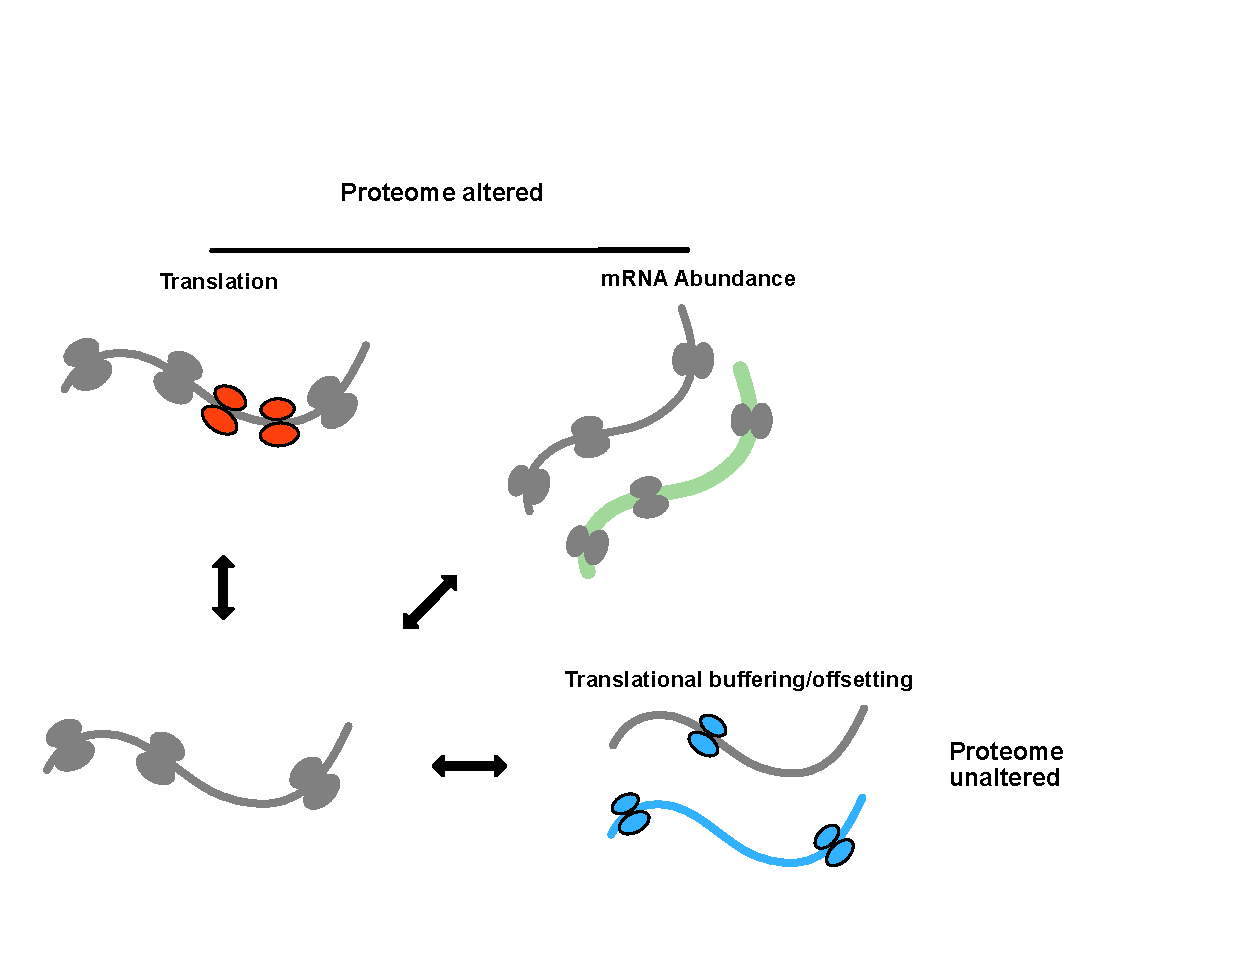
\includegraphics{./figures/geneModes_MRNA.pdf}
  \caption{Regulatory modes of gene expression - Schematic representation of regulatory modes of translation efficiency in a fold-change scatter plot. Indicated in red are changes in translation (i.e. changes in translated mRNA but not total mRNA), in green changes in mRNA abundance (i.e. congruent changes between total mRNA and translated mRNA) and in blue translational buffering (i.e. changes in total mRNA levels but not translated mRNA levels). TE changes as the TE-score would estimate them are indicated.\label{fig:mRNA}}
\end{wrapfigure}

In recent years, evidence emerged where translation efficiencies of
mRNAs can be altered to compensate for changes in total mRNA levels.
Within this newly identified mode of regulation of mRNA translation
``translational buffering'', mRNA translation is altered such that
changes in total mRNA levels do not influence their corresponding
protein levels (Oertlin et al., 2019,McManus, May, Spealman, \& Shteyman
(2014),Lorent et al. (2019)). Translational buffering is observed to
compensate for inter-tissue, inter-species and inter-individual
difference (Artieri \& Fraser, 2014,C. Cenik et al. (2015),Perl et al.
(2017)). Furthermore, in bacteria translational buffering maintains
protein complex stoichiometry as well as protein levels for conserved
pathway across species (G.-W. Li, Burkhardt, Gross, \& Weissman,
2014,Lalanne et al. (2018)). Recently translational buffering has been
observed under conditions where estrogen receptor alpha (ERalpha) is
depleted. ERalpha modulates activity of specific tRNA modification
enzymes. These enzymes are needed for the U34 tRNA modification. Loss of
ERalpha led to reduced U34 tRNA modification thereby hindering
translation of mRNAs requiring such modified tRNAs. For these mRNAs,
even though their total mRNA levels were induced across conditions,
their protein levels remained constant (Lorent et al., 2019). Given
these multiple roles of mRNA translation to regulate the proteome it is
critical to distinguish them as their underlying mechanisms can have
different biological implications.

\section{Expertimental methods to measure mRNA translation}

\subsection{Polysome profiling}

is a technique to measure changes in translational efficiencies of mRNAs
between two or more conditions. Polysome profiling allows for separation
of polysomes from monosomes, ribosomal subunits and messenger
ribonucleoprotein particles (mRNPs). During the assay, ribosomes are
immobilized on the mRNAs using translation elongation inhibitors
(e.g.~cycloheximide). Cytoplasmic RNA extracts are then sedimented on a
linear sucrose gradient (5-50\%) using ultra centrifugation.

\begin{wrapfigure}{r}{0.6\textwidth}
    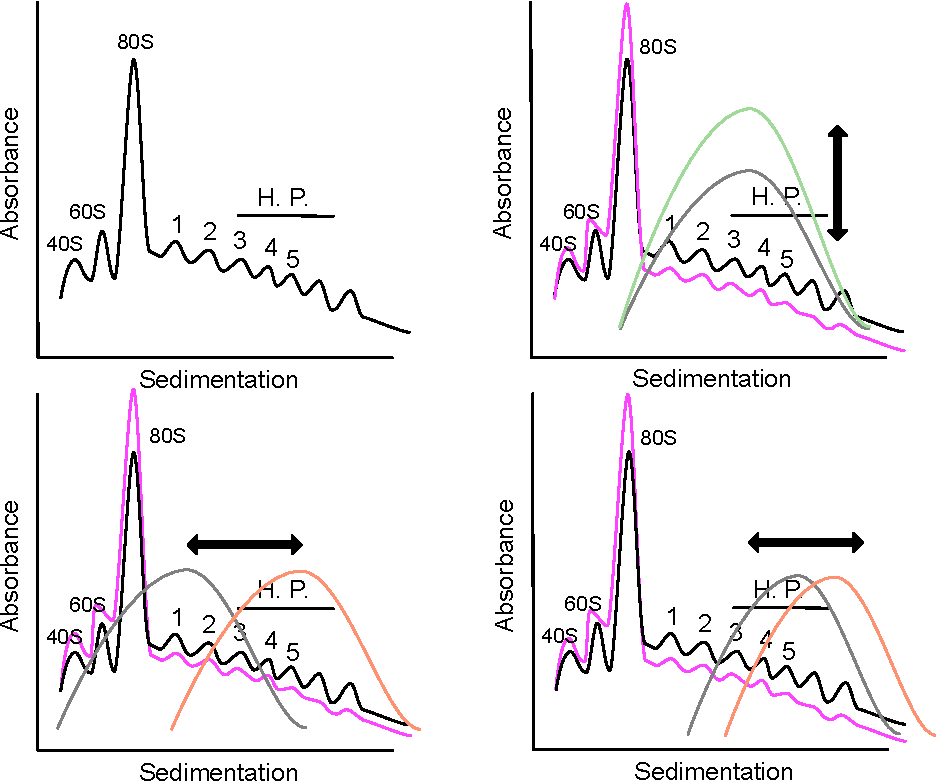
\includegraphics[width=0.9\linewidth]{./figures/polysome_shifts.pdf}
  \caption{Polysome profliles -  (top left) Schematic representation of a polysome profile using linear sucrose gradient fractionation. Indicated in the polysome profiles are the 40S, 60S ribosomal subunits as well as the 80S monosome. H.P. indicates heavy polysome fractions.Between conditions distribution changes for mRNA abundance (top right), translation (bottom left) and translation within high polysome fractions (bottom right) are illustrated. \label{fig:polysome}}
\end{wrapfigure}

The resulting gradient is fractionated and mRNAs with different number
of bound ribosomes can be extracted and analyzed for changes in
translational efficiency (Gandin et al., 2014). An illustration of a
polysome profile with peaks for the 40S, 60S subunits and 80S ribosome
can be seen in (\textbf{Fig \ref{fig:polysome} top left}). Subsequent
peaks along the frations indicate the mRNAs with 1 or more bound
ribosome. mRNAs are typically normally distributed along the fractions,
i.e.~a pool of the same mRNA will be associated with 1- n number of
ribosomes. Changes in mRNA abundance will lead to an overall increase in
the amount of isolated polysome-associated mRNA without a shift of the
distribution along the fractions (\textbf{Fig \ref{fig:polysome} top
right}). This means that the translation efficiency per mRNA remains
unchanged. Changes in translational efficiency can be observed by shifts
of polysome association for mRNAs from the light (inefficiently
translated) towards the heavy (efficiently translated) polysome
fractions or vice versa (\textbf{Fig \ref{fig:polysome} bottom left}).
Shift within the heavy polysome fractions (i.e.~3 bound ribosome to 7
bound ribosome) can also occur (\textbf{Fig \ref{fig:polysome} bottom
right}). These shift remain undetected in cases where the distribtion of
polysome-associated mRNAs does not sufficiently shift across the
fractions and is a limitation of polysome profiling. Quantification of
mRNA levels within each fraction can be assessed using Northern blotting
or reverse transcription quantitative polymerase chain reaction
(RT-qPCR). For transcriptome wide studies, pooling of efficiently
translated mRNAs (mRNAs with \textgreater{}3 bound ribosomes) followed
by quantification using either DNA-microarrays or RNA sequencing is
common. Pooling of mRNAs as well as collection of multiple fractions
makes polysome profiling inconvenient when dealing with large samples
sizes or experiments with low amounts of input RNA. Therefore, an
optimized sucrose gradient was developed where most efficiently
translated mRNAs are collected on a sucrose cushion and thereby can be
isolated from one single fraction (Liang et al., 2018). This optimized
gradient allows for application of polysome profiling in small tissue
samples where RNA quantity is limiting and reduces labor intensity of
the assay. Polysome-associated mRNA levels are subject to changes in
translation efficiency as well as factors contributing to cytosolic mRNA
levels. Mechanisms such as transcription (i.e.~in the case of mRNA
abundance) or mRNA stability can affect cytosolic mRNA levels which
impacts the pool of mRNAs that can be associated to polysomes.
Therefore, to identify bona fide changes in translation efficiency it is
important to collect cytoplasmic mRNA levels in parallel to
polysome-associated mRNA to correct for such mechanisms
(e.g.~transcription or mRNA stability) during downstream analysis
(Gandin et al., 2014,Oertlin et al. (2019)).

\subsection{Ribosome profiling} \label{riboseq}

is a technique that enables sequencing of ribosome protected mRNA
fragments (RPFs). In the assay ribosomes are immobilized on the mRNAs
using, similar to polysome profiling, translation elongations inhibitors
(e.g.~cyclohexamide) (Ingolia, 2010,Ingolia (2016)). One limitation with
the use of translation elongation inhibitors is the distortion of
ribosome distributions especially at translation initiation sites. These
introduced artefacts need to be accounted for in the downstream analysis
when assessing ribosome position along the mRNA. Following the
translation elongation inhibitor treatment, cells ought to be
immediately flash frozen using liquid nitrogen. Alternatively, using
only flash freezing has been seen as a robust approach in a wide range
of diverse organisms (Brar \& Weissman, 2015). Generation of RPFs is
achieved by RNAse treatment breaking the links of RNA between ribosomes
leaving single ribosomes with a \textasciitilde{}28 nucleotide long RNA
fragment within each ribosome. RPFs are then isolated using ultra
centrifugation through a sucrose cushion. Co-migration of RNA fragments
such as structured non-coding RNAs or large ribonucleoprotein complexes
within the sucrose gradient can be a cause of contamination and thereby
can provide false readouts of translation. A polyacrylamide gel loaded
with RPFs and a reference ladder is used to select RPFs of the right
size. Typically, RPFs with lengths of 25 to 30 nucleotides are selected.
The RPFs can then be pooled if sample specific barcodes are used. After
size selection a pre-adenylated DNA is ligated to the RPFs. This RNA-DNA
construct is then used as template for reverse transcription. Through
gel-based purification, full-length products of the reverse
transcription are selected and circularized. Following circularization,
a double stranded DNA library is constructed and PCR amplified. This
library is suitable for quantification using RNAseq. In parallel to RPF
selection, randomly fragmented total mRNA of the same size is also
retrieved. This is achieved by extraction of total mRNA from cell lysate
followed by purification via recovery of polyadenylated messages or
removal of ribosomal RNA. Fragmentation of total RNA is done using an
alkaline fragmentation buffer (Ingolia, 2010,Brar \& Weissman (2015)).

\subsection{Comparing ribosome and polysome profiling}

Albeit both methods generate count data after quantification with
RNAsequencing, there are some key aspects that differ between the
techniques. Polysome profiling separates efficiently translated mRNAs
from non- efficiently translated mRNAs along a sucrose thereby creating
an mRNA based perspective for analyzing changes in translational
efficiencies. In contrast, ribosome profiling determines translational
efficiencies by counting the number of RPFs of both efficiently and
non-efficiently translated mRNAs. Changes in translational efficiencies,
e.g.~shifts between the polysomal fractions, can be dramatic (I.e. near
complete dissociation of ribosomes from an mRNA) or subtle (shifts from
2 to 4 ribosomes) (Livingstone et al., 2015). Ribosome profiling has
been shown to be biased towards identification of dramatic shifts of
associated ribosomes to mRNAs, whereas subtle shifts are masked which
can lead to false biological conclusions. Polysome profiling is affected
by this to a much lesser extent, thereby more robust in identifying such
changes (Masvidal et al., 2017). RPFs in ribosome profiling provide
exact nucleotide positions occupied by ribosomes thereby offering single
nucleotide resolution. Polysome profiling cannot reveal ribosome
locations along the mRNA. However, polysome profiling allows access to
full-length mRNAs that includes the UTRs. The single nucleotide
resolution of ribosome profiling is necessary in contexts studying local
translation events such as ribosomal frame shifts (Rato, Amirova, Bates,
Stansfield, \& Wallace, 2011) or uORF translation (Andreev et al.,
2015). Higher sensitivity in detecting changes in translational
efficiencies on a global scale makes polysome profiling more suitable
for transcriptome-wide studies (Gandin et al., 2016a). Both methods have
their strengths and weaknesses and therefore each method should be
considered depending on the underlying biological question of each
experiment.

\section{Algorithms for analysis of changes in translation efficiencies}

In polysome-profiling and ribosome profiling translated mRNAs
(i.e.~polysome-associated mRNAs and RPFs) are separated in parallel from
their total mRNA counterpart. Estimating translation efficiencies
requires that changes in translated mRNA are corrected for changes in
total mRNA to accurately identify the regulatory modes of gene
expression (i.e.~translation, mRNA abundance and translational
buffering)(Oertlin et al., 2019). Here we will discuss methods that
analyse polysome-profiling and ribosome profiling data to estimate
changes in translation efficiencies across 2 or more conditions and how
these methods identify different regulatory modes of gene expression.

Initially analysis of transcriptome-wide translation studies used an
approach called the translation efficiency (TE-score) that uses the
following equation:
\[\varDelta TE = \frac{\frac{P_{c2}}{T_{c2}}} {\frac{P_{c1}}{T_{c1}}}\\\]

This score calculates the ratio of the ratios between
polysome-associated mRNA levels (P) divided by total mRNA levels (T)
within each condition (i.e.~C1 and C2). The TE- score approach has been
shown to be prone to spurious correlations (Larsson, Sonenberg, \&
Nadon, 2010). Spurious correlations arise due to that the ratio of
polysome-associated mRNA and total mRNA can systematically correlate
with total mRNA levels which is not corrected for in this equation and
leads to an elevated type-1 error. \clearpage

\begin{wrapfigure}{o}{0.5\textwidth}
  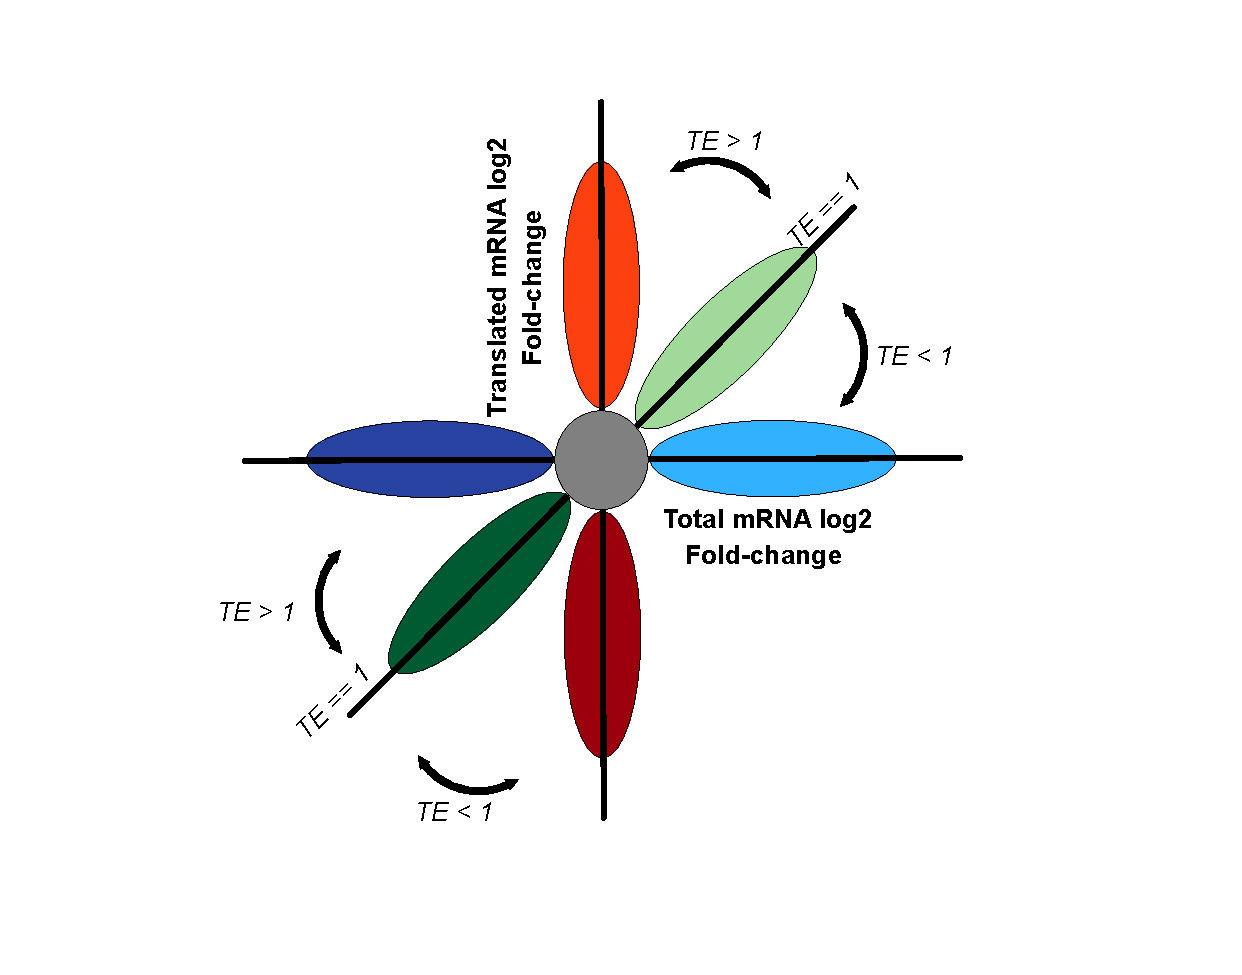
\includegraphics{./figures/geneModes_TE.pdf}
  \caption{TE scores for regulatory modes of gene expression -  Schematic representation of regulatory modes of translation efficiency in a fold-change scatter plot. Indicated in red are changes in translation efficiency altering protein levels, in green changes in mRNA abundance and in blue changes in translation efficiency leading to translational buffering/offsetting. The shifts for the translation efficiency (TE) score are indicated. \label{fig:TE}}
\end{wrapfigure}

\textbf{Figure \ref{fig:TE}} gives an overview of the relationship
between a change in TE) and each regulatory mode of gene expression.
Changes in mRNA abundance will lead to a \(\varDelta\)TE close to 0 in
log space (i.e.~no change) as total mRNA and translated mRNA change with
a similar magnitude. However, in the case of both translation and
translational buffering, terms in the TE-score equation change leading
to a \(\varDelta\)TE (TE \textless{} 0 or TE \textgreater{} 0) and
thereby identification of both changes in translation and translational
buffering simultaneously. Therefore, the TE-score method fails to
differentiate between changes in translation and translational buffering
which can have drastic consequences for the biological interpretation of
the results (Oertlin et al., 2019).

The TE-score approach was challenged by the Analysis of Translation
Activity (anota) algorithm which was developed for DNA-microarray data
(Larsson, Sonenberg, \& Nadon, 2011). anota combines analysis of partial
variance (APV)(Schleifer, Eckholdt, Cohen, \& Keller, 1993) with a
random variance model (RVM)(Wright \& Simon, 2003). RVM estimates gene
variance using shared informatio across all genes to increase power for
detection of differential expression(Wright \& Simon, 2003). anota uses
a two-step process that firstly assesses the model assumptions for (i)
absence of highly influential data points, (ii) common slopes of sample
classes, (iii) homoscedasticity of residuals and (iv) normal
distribution of per gene residuals. In the second step then performs
analysis of changes in translational activity using the following model:

\[log(y_{gi}) = \beta_g^{RNA}\ X_i^{RNA}+ \beta_g^{cond}\ X_i^{cond} + \varepsilon_{gi}\]

here \(\beta_g^{RNA}\) described the relationship to total RNA \(gth\)
gene \(ith\) sample of model matrix \(X\); \(\beta_g^{cond}\) represent
the log2 fold change for treatment classes and \(\varepsilon_{gi}\)
denotes the residual error.

\begin{wrapfigure}{o}{0.5\textwidth}
  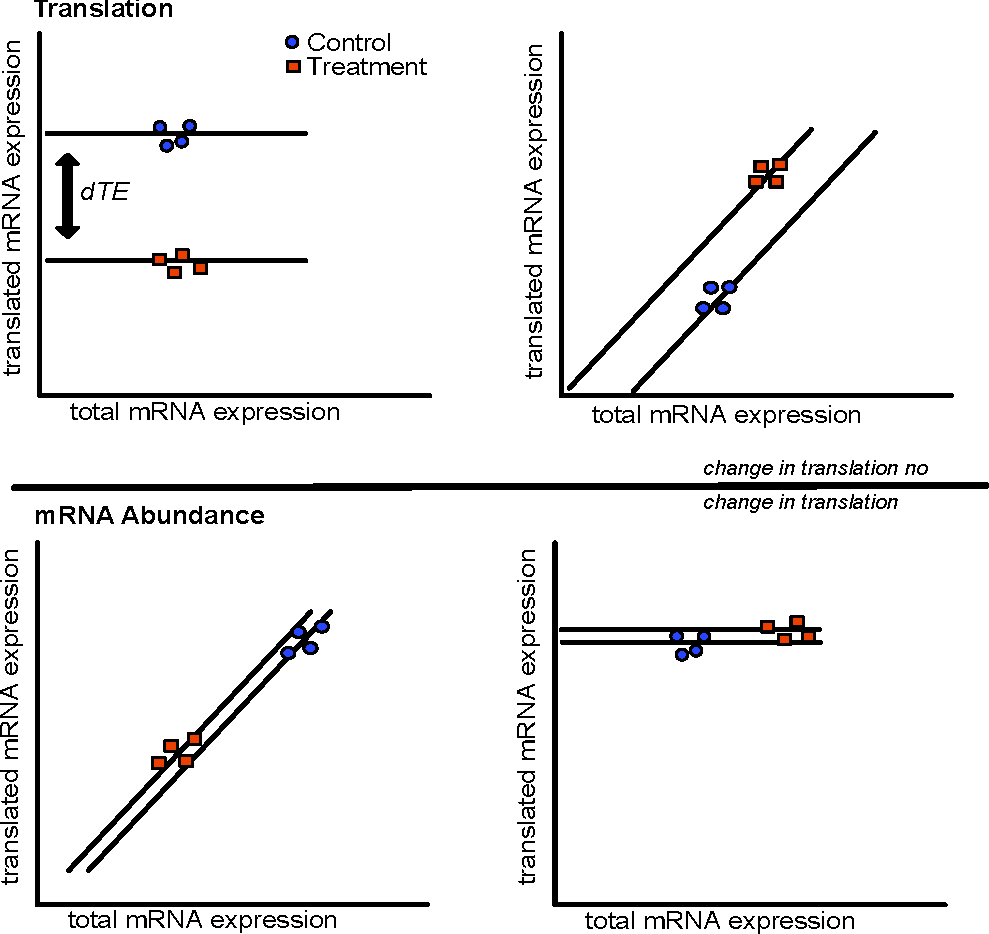
\includegraphics{./figures/geneModes_anota_Larsson.pdf}
  \caption{anota gene models - Schematic representation of the anota analysis models. Translation mRNA expression is set out against total mRNA expression for each biological replicate and treatment condition. Top left shows the model of a gene that is differentially translated (i.e. change in translated but not total mRNA). The difference in the slope intercepts are used to estimate changes in translation efficiencies between conditions i.e. dTE. Other gene models are shown; change in translation efficiency with varying total mRNA levels (top right); change in mRNA abundance (bottom left) and translational buffering (bottom right).
  \label{fig:anota}}
\end{wrapfigure}

Within anota a common slope for the treatment classes that describes the
translated mRNA to total mRNA relationship is calculated. The difference
between the slope intercepts is then interpreted as the \(\varDelta\)
TE. A simplified view of this model can be seen in (\textbf{Figure
\ref{fig:anota} top left}). Here expression for translated mRNA and
total mRNA are modeled over two sample classes with each 4 replicates.
Furthermore, changes in translation efficiencies can also be observed
when translated mRNAs shift to a larger extent than the total mRNA
levels (\textbf{Figure \ref{fig:anota} top right}). Identification of
genes in this categorie can be a challenge, especially in highyl
variable data set, as they resemble mRNA abundance genes (\textbf{Figure
\ref{fig:anota} bottom left}). Nevertheless, Using the linear regression
analysis anota accurately corrects changes in translated mRNA as can be
seen in (\textbf{Figure \ref{fig:anota} bottom right}) where a change in
total mRNA but not translated mRNA levels is observed. For this gene the
difference in slope intercepts is small and will not be identified as
difference in translation as would be the case in the TE-score approach.
anota was developed at a time where translational buffering was
uncommonly seen in data sets. Naturally, the methods lacks a setting to
analyse translational buffering. This was addressed in anota's
successor, anota2seq, and will be discussed in \textbf{Study 1}.

Advances in experimental methods warrant for appropriate statistical
methods to analyse data resulting from them. DNA- microarray was the
dominant platform to assess genome-wide changes before the advent of RNA
sequencing. In DNA- microarray RNA hybridizes probes on a chip and
generate a signal of which the measured intensity is an indicator of
expression, whereas in RNA sequencing reads from RNAs are counted.
Intensity data from DNA microarray can be normalised and transformed
(i.e.~log transformation) to fulfill the requirements for application of
linear models, whereas RNA sequencing harbours additional
characteristics that need to be accounted for. Therefore, algorithms
developed for analysis of DNA- microarray are not directly applicable to
RNA sequencing data as is the case for the anota algorithm.

RNA sequencing data shows variance that is greater than the mean which
is commonly referred to as overdispersion. Count data from RNA
sequencing have been initially approached using Poisson distributions
which assumes that the variance is equal to the mean(J. Lu et al.,
2005). Now established RNA sequencing analysis frameworks such as edgeR
and DESeq2 use negative binomial distributions in combination with
generalized linear models (GLMs) (Robinson, McCarthy, \& Smyth, 2010,
Love, Huber, \& Anders (2014)). The negative binomial distribution uses
a dispersion parameter to account for overdispersion (McCarthy, Chen, \&
Smyth, 2012). While analysis principles of DESeq2 and edgeR are similar
they differ in their normalisation method, dispersion estimation and
information sharing across genes. In a simple differential expression
analysis between two conditions with one RNA type the GLM model would be
as in the following equation:

\[log(y_{gi}) = \beta_g^{cond}\ X_i^{cond} + \varepsilon_{gi}\]

here \(\beta_g^{cond}\ X_i^{cond}\) represent the condition
(i.e.~control and treatment) log2 fold change for the \(gth\) gene
\(ith\) sample of the model matrix X and \(\varepsilon_{gi}\) denotes
the residual error. When analysing changes in translation effiencies
additional parameter for RNA type (i.e.~total mRNA or translated mRNA)
and the interaction between the RNA type and condition are added so
that:

\[log(y_{gi}) = \beta_g^{RNA}\ X_i^{RNA}+ \beta_g^{cond}\ X_i^{cond} + \beta_g^{RNA:cond}\ X_i^{interaction} + \varepsilon_gi\]

In this model the interaction term is interpreted as the change in
translation effiencies (Chothani et al., 2019). Other methods
(i.e.~Ribodiff(Zhong et al., 2017), Riborex(W. Li, Wang, Uren, Penalva,
\& Smith, 2017) and deltaTE (Chothani et al., 2019)) borrow this
analysis principle of an GLM with an interaction term by often applying
this exact model. A noteable difference is that Ribodiff allows
dispersion estimation for translated mRNA and total mRNA separetly as
variance differences between the RNA types can be expected due to
varying experimental protocols (Zhong et al., 2017, Liang et al.
(2018)). While the flexibility of GLMs allows for complex study designs
involving 2 or more treatment conditions, Riborex and Ribodiff limit the
study design to only two conditions. DeltaTE gives their users full
flexibility of the DESeq2 GLM model. Xtail is a method developed for
ribosome profiling that makes use of DESeq2 for RNAseq count
normalisation (Xiao, Zou, Liu, \& Yang, 2016). Their assessment of
differences in translation efficiencies relies on probability matrices
for the ratio of translated mRNA over total mRNA within condition and a
between condition ratio of these ratios. Babel was the first algorithm
designed solely for analysis of differential translation and uses an
error-in-varaibles regression analysis (A. B. Olshen et al., 2013). The
error-in- variables regression allows accounting for variable total mRNA
levels when assessing changes in translation. Although these methods
have distinct approaches to identify changes in translation
efficiencies, their principle of analysis is similar to comparing a
ratio of ratios. Therefore these methods suffer from similar issues as
the TE-score which will be discussed in \textbf{Study 1}.

\chapter{Aims of this thesis}

The aims of this thesis are to expand current methodologies for analysis
of translation efficiency data and explore the regulation of gene
expression in cancer.

In \textbf{Study I} we adapted an algorithm for ANalysis Of Translation
Activity data (anota) so that it could be applied to next generation
sequencing data. Furthermore, we implemented the analysis of
translational buffering a recently described regulatory mode of gene
expression. The resulting algorithm was named anota2seq.

We then applied the anota2seq algorithm to investigate changes in
translation efficiencies in two cancer models:

In \textbf{Study II} we unravelled the effects of eIF4A, an RNA
helicase, inhibition using a synthetic rocaglate CR-1-31-B (CR-31) in
pancreatic ductal adenocarcinoma.

In \textbf{Study III} we explored the effects of insulin on gene
expression in multiple cell lines.

\chapter{Results and discussion}

\chapter{Conclusions}

\chapter*{Acknowledgments}\label{acknowledgments}
\addcontentsline{toc}{chapter}{Acknowledgments}

\chapter*{References}\label{references}
\addcontentsline{toc}{chapter}{References}

\hypertarget{refs}{}
\hypertarget{ref-Afonina2014}{}
Afonina, Z. A., Myasnikov, A. G., Shirokov, V. A., Klaholz, B. P., \&
Spirin, A. S. (2014). Formation of circular polyribosomes on eukaryotic
mRNA without cap-structure and poly(A)-tail: A cryo electron tomography
study. \emph{Nucleic Acids Research}, \emph{42}(14), 9461--9469.
\url{https://doi.org/10.1093/nar/gku599}

\hypertarget{ref-Alkalaeva2006}{}
Alkalaeva, E. Z., Pisarev, A. V., Frolova, L. Y., Kisselev, L. L., \&
Pestova, T. V. (2006). In Vitro Reconstitution of Eukaryotic Translation
Reveals Cooperativity between Release Factors eRF1 and eRF3.
\emph{Cell}, \emph{125}(6), 1125--1136.
\url{https://doi.org/10.1016/j.cell.2006.04.035}

\hypertarget{ref-Amrani2008}{}
Amrani, N., Ghosh, S., Mangus, D. A., \& Jacobson, A. (2008).
Translation factors promote the formation of two states of the
closed-loop mRNP. \emph{Nature}, \emph{453}(7199), 1276--1280.
\url{https://doi.org/10.1038/nature06974}

\hypertarget{ref-Andreev2015}{}
Andreev, D. E., O'Connor, P. B., Fahey, C., Kenny, E. M., Terenin, I.
M., Dmitriev, S. E., \ldots{} Baranov, P. V. (2015). Translation of
5\({'}\) leaders is pervasive in genes resistant to eIF2 repression.
\emph{ELife}, \emph{4}, e03971.
\url{https://doi.org/10.7554/eLife.03971}

\hypertarget{ref-Artieri2014}{}
Artieri, C. G., \& Fraser, H. B. (2014). Evolution at two levels of gene
expression in yeast. \emph{Genome Research}, \emph{24}(3), 411--421.
\url{https://doi.org/10.1101/gr.165522.113}

\hypertarget{ref-Asano2000}{}
Asano, K., Clayton, J., Shalev, A., \& Hinnebusch, A. G. (2000). A
multifactor complex of eukaryotic initiation factors, eIF1, eIF2, eIF3,
eIF5, and initiator tRNAMet is an important translation initiation
intermediate in vivo. \emph{Genes \& Development}, \emph{14}(19),
2534--2546. \url{https://doi.org/10.1101/gad.831800}

\hypertarget{ref-Baou2011}{}
Baou, M., Norton, J. D., \& Murphy, J. J. (2011). AU-rich RNA binding
proteins in hematopoiesis and leukemogenesis. \emph{Blood},
\emph{118}(22), 5732--5740.
\url{https://doi.org/10.1182/blood-2011-07-347237}

\hypertarget{ref-Brar2015}{}
Brar, G. A., \& Weissman, J. S. (2015). Ribosome profiling reveals the
what, when, where and how of protein synthesis. \emph{Nature Reviews.
Molecular Cell Biology}, \emph{16}(11), 651--664.
\url{https://doi.org/10.1038/nrm4069}

\hypertarget{ref-Buttgereit1995}{}
Buttgereit, F., \& Brand, M. D. (1995). A hierarchy of ATP-consuming
processes in mammalian cells. \emph{The Biochemical Journal}, \emph{312
( Pt 1)}(Pt 1), 163--7. \url{https://doi.org/10.1042/bj3120163}

\hypertarget{ref-Calvo2009}{}
Calvo, S. E., Pagliarini, D. J., \& Mootha, V. K. (2009). Upstream open
reading frames cause widespread reduction of protein expression and are
polymorphic among humans. \emph{Proceedings of the National Academy of
Sciences}, \emph{106}(18), 7507--7512.
\url{https://doi.org/10.1073/pnas.0810916106}

\hypertarget{ref-Cenik2015}{}
Cenik, C., Cenik, E. S., Byeon, G. W., Grubert, F., Candille, S. I.,
Spacek, D., \ldots{} Snyder, M. P. (2015). Integrative analysis of RNA,
translation, and protein levels reveals distinct regulatory variation
across humans. \emph{Genome Research}, \emph{25}(11), 1610--1621.
\url{https://doi.org/10.1101/gr.193342.115}

\hypertarget{ref-Cheng2016}{}
Cheng, Z., Teo, G., Krueger, S., Rock, T. M., Koh, H. W. L., Choi, H.,
\& Vogel, C. (2016). Differential dynamics of the mammalian mRNA and
protein expression response to misfolding stress. \emph{Molecular
Systems Biology}, \emph{12}(1), 855.
\url{https://doi.org/10.15252/msb.20156423}

\hypertarget{ref-Chothani2019}{}
Chothani, S., Adami, E., Ouyang, J. F., Viswanathan, S., Hubner, N.,
Cook, S. A., \ldots{} Rackham, O. J. L. (2019). deltaTE: Detection of
Translationally Regulated Genes by Integrative Analysis of Ribo-seq and
RNA-seq Data. \emph{Current Protocols in Molecular Biology},
\emph{129}(1), e108. \url{https://doi.org/10.1002/cpmb.108}

\hypertarget{ref-Crick1970}{}
Crick, F. (1970). Central Dogma of Molecular Biology. \emph{Nature},
\emph{227}(5258), 561--563. \url{https://doi.org/10.1038/227561a0}

\hypertarget{ref-deSousaAbreu2009}{}
de Sousa Abreu, R., Penalva, L. O., Marcotte, E. M., \& Vogel, C.
(2009). Global signatures of protein and mRNA expression levels.
\emph{Molecular BioSystems}, \emph{5}(12), 1512--1526.
\url{https://doi.org/10.1039/b908315d}

\hypertarget{ref-Denkert2004}{}
Denkert, C., Weichert, W., Winzer, K.-J., Müller, B.-M., Noske, A.,
Niesporek, S., \ldots{} Hauptmann, S. (2004). Expression of the
ELAV-Like Protein HuR Is Associated with Higher Tumor Grade and
Increased Cyclooxygenase-2 Expression in Human Breast Carcinoma.
\emph{Clinical Cancer Research}, \emph{10}(16), 5580--5586.
\url{https://doi.org/10.1158/1078-0432.CCR-04-0070}

\hypertarget{ref-Dever2012}{}
Dever, T. E., \& Green, R. (2012). The elongation, termination, and
recycling phases of translation in eukaryotes. \emph{Cold Spring Harbor
Perspectives in Biology}, \emph{4}(7), 1--16.
\url{https://doi.org/10.1101/cshperspect.a013706}

\hypertarget{ref-Dorner2006}{}
Dorner, S., Brunelle, J. L., Sharma, D., \& Green, R. (2006). The hybrid
state of tRNA binding is an authentic translation elongation
intermediate. \emph{Nature Structural \& Molecular Biology},
\emph{13}(3), 234--241. \url{https://doi.org/10.1038/nsmb1060}

\hypertarget{ref-Fan1998}{}
Fan, X. C., \& Steitz, J. A. (1998). Overexpression of HuR, a
nuclearCytoplasmic shuttling protein, increases the in vivo stability of
ARE-containing mRNAs. \emph{The EMBO Journal}, \emph{17}(12),
3448--3460. \url{https://doi.org/10.1093/emboj/17.12.3448}

\hypertarget{ref-Gandin2016}{}
Gandin, V., Masvidal, L., Cargnello, M., Gyenis, L., McLaughlan, S.,
Cai, Y., \ldots{} Topisirovic, I. (2016a). mTORC1 and CK2 coordinate
ternary and eIF4F complex assembly. \emph{Nature Communications},
\emph{7}(1), 11127. \url{https://doi.org/10.1038/ncomms11127}

\hypertarget{ref-Gandin2016a}{}
Gandin, V., Masvidal, L., Hulea, L., Gravel, S.-P., Cargnello, M.,
McLaughlan, S., \ldots{} Topisirovic, I. (2016b). nanoCAGE reveals 5'
UTR features that define specific modes of translation of functionally
related MTOR-sensitive mRNAs. \emph{Genome Research}, \emph{26}(5),
636--648. \url{https://doi.org/10.1101/gr.197566.115}

\hypertarget{ref-Gandin2014}{}
Gandin, V., Sikström, K., Alain, T., Morita, M., McLaughlan, S.,
Larsson, O., \& Topisirovic, I. (2014). Polysome fractionation and
analysis of mammalian translatomes on a genome-wide scale. \emph{Journal
of Visualized Experiments: JoVE}, (87).
\url{https://doi.org/10.3791/51455}

\hypertarget{ref-Graff2009}{}
Graff, J. R., Konicek, B. W., Lynch, R. L., Dumstorf, C. A., Dowless, M.
S., McNulty, A. M., \ldots{} Carter, J. H. (2009). eIF4E activation is
commonly elevated in advanced human prostate cancers and significantly
related to reduced patient survival. \emph{Cancer Research},
\emph{69}(9), 3866--3873.
\url{https://doi.org/10.1158/0008-5472.CAN-08-3472}

\hypertarget{ref-Grifo1983}{}
Grifo, J. A., Tahara, S. M., Morgan, M. A., Shatkin, A. J., \& Merrick,
W. C. (1983). New initiation factor activity required for globin mRNA
translation. \emph{Journal of Biological Chemistry}, \emph{258}(9),
5804--5810. \url{https://doi.org/10.1016/S0021-9258(20)81965-6}

\hypertarget{ref-Guan2017}{}
Guan, B.-J., van Hoef, V., Jobava, R., Elroy-Stein, O., Valasek, L. S.,
Cargnello, M., \ldots{} Hatzoglou, M. (2017). A Unique ISR Program
Determines Cellular Responses to Chronic Stress. \emph{Molecular Cell},
\emph{68}(5), 885--900.e6.
\url{https://doi.org/10.1016/j.molcel.2017.11.007}

\hypertarget{ref-Heerlein2005}{}
Heerlein, K., Schulze, A., Hotz, L., Bärtsch, P., \& Mairbäurl, H.
(2005). Hypoxia decreases cellular ATP demand and inhibits mitochondrial
respiration of a549 cells. \emph{American Journal of Respiratory Cell
and Molecular Biology}, \emph{32}(1), 44--51.
\url{https://doi.org/10.1165/rcmb.2004-0202OC}

\hypertarget{ref-Hellen2018}{}
Hellen, C. U. T. (2018). Translation Termination and Ribosome Recycling
in Eukaryotes. \emph{Cold Spring Harbor Perspectives in Biology},
\emph{10}(10), a032656.
\url{https://doi.org/10.1101/cshperspect.a032656}

\hypertarget{ref-Hinnebusch2006}{}
Hinnebusch, A. G. (2006). eIF3: A versatile scaffold for translation
initiation complexes. \emph{Trends in Biochemical Sciences},
\emph{31}(10), 553--562.
\url{https://doi.org/10.1016/j.tibs.2006.08.005}

\hypertarget{ref-Ingolia2010}{}
Ingolia, N. T. (2010). Genome-wide translational profiling by ribosome
footprinting. \emph{Methods in Enzymology}, \emph{470}, 119--142.
\url{https://doi.org/10.1016/S0076-6879(10)70006-9}

\hypertarget{ref-Ingolia2016}{}
Ingolia, N. T. (2016). Ribosome Footprint Profiling of Translation
throughout the Genome. \emph{Cell}, \emph{165}(1), 22--33.
\url{https://doi.org/10.1016/j.cell.2016.02.066}

\hypertarget{ref-Ingolia2011}{}
Ingolia, N. T., Lareau, L. F., \& Weissman, J. S. (2011). Ribosome
Profiling of Mouse Embryonic Stem Cells Reveals the Complexity and
Dynamics of Mammalian Proteomes. \emph{Cell}, \emph{147}(4), 789--802.
\url{https://doi.org/10.1016/j.cell.2011.10.002}

\hypertarget{ref-Inoki2003}{}
Inoki, K., Zhu, T., \& Guan, K.-L. (2003). TSC2 mediates cellular energy
response to control cell growth and survival. \emph{Cell},
\emph{115}(5), 577--590.
\url{https://doi.org/10.1016/s0092-8674(03)00929-2}

\hypertarget{ref-Iwasaki2016}{}
Iwasaki, S., Floor, S. N., \& Ingolia, N. T. (2016). Rocaglates convert
DEAD-box protein eIF4A into a sequence-selective translational
repressor. \emph{Nature}, \emph{534}(7608), 558--561.
\url{https://doi.org/10.1038/nature17978}

\hypertarget{ref-Jackson1991}{}
Jackson, R. J. (1991). The ATP requirement for initiation of eukaryotic
translation varies according to the mRNA species. \emph{European Journal
of Biochemistry}, \emph{200}(2), 285--294.
\url{https://doi.org/10.1111/j.1432-1033.1991.tb16184.x}

\hypertarget{ref-Jia2021}{}
Jia, J.-J., Lahr, R. M., Solgaard, M. T., Moraes, B. J., Pointet, R.,
Yang, A.-D., \ldots{} Fonseca, B. D. (2021). mTORC1 promotes TOP mRNA
translation through site-specific phosphorylation of LARP1.
\emph{Nucleic Acids Research}.
\url{https://doi.org/10.1093/nar/gkaa1239}

\hypertarget{ref-JolyAnne-Laure2018}{}
Joly Anne-Laure, Seitz Christina, Liu Sang, Kuznetsov Nikolai V., Gertow
Karl, Westerberg Lisa S., \ldots{} Andersson John. (2018). Alternative
Splicing of FOXP3 Controls Regulatory T Cell Effector Functions and Is
Associated With Human Atherosclerotic Plaque Stability.
\emph{Circulation Research}, \emph{122}(10), 1385--1394.
\url{https://doi.org/10.1161/CIRCRESAHA.117.312340}

\hypertarget{ref-Jovanovic2015}{}
Jovanovic, M., Rooney, M. S., Mertins, P., Przybylski, D., Chevrier, N.,
Satija, R., \ldots{} Regev, A. (2015). Dynamic profiling of the protein
life cycle in response to pathogens. \emph{Science}, \emph{347}(6226).
\url{https://doi.org/10.1126/science.1259038}

\hypertarget{ref-Kapur2017}{}
Kapur, M., Monaghan, C. E., \& Ackerman, S. L. (2017). Regulation of
mRNA Translation in Neurons-A Matter of Life and Death. \emph{Neuron},
\emph{96}(3), 616--637.
\url{https://doi.org/10.1016/j.neuron.2017.09.057}

\hypertarget{ref-Kimball2006}{}
Kimball, S. R. (2006). Interaction between the AMP-Activated Protein
Kinase and mTOR Signaling Pathways. \emph{Medicine \& Science in Sports
\& Exercise}, \emph{38}(11), 1958--1964.
\url{https://doi.org/10.1249/01.mss.0000233796.16411.13}

\hypertarget{ref-Kozak1984}{}
Kozak, M. (1984). Compilation and analysis of sequences upstream from
the translational start site in eukaryotic mRNAs. \emph{Nucleic Acids
Research}, \emph{12}(2), 857--872.
\url{https://doi.org/10.1093/nar/12.2.857}

\hypertarget{ref-Kozak1986}{}
Kozak, M. (1986). Point mutations define a sequence flanking the AUG
initiator codon that modulates translation by eukaryotic ribosomes.
\emph{Cell}, \emph{44}(2), 283--292.
\url{https://doi.org/10.1016/0092-8674(86)90762-2}

\hypertarget{ref-Lalanne2018}{}
Lalanne, J.-B., Taggart, J. C., Guo, M. S., Herzel, L., Schieler, A., \&
Li, G.-W. (2018). Evolutionary Convergence of Pathway-Specific Enzyme
Expression Stoichiometry. \emph{Cell}, \emph{173}(3), 749--761.e38.
\url{https://doi.org/10.1016/j.cell.2018.03.007}

\hypertarget{ref-Larsson2010}{}
Larsson, O., Sonenberg, N., \& Nadon, R. (2010). Identification of
differential translation in genome wide studies. \emph{Proceedings of
the National Academy of Sciences}, \emph{107}(50), 21487--21492.
\url{https://doi.org/10.1073/pnas.1006821107}

\hypertarget{ref-Larsson2011}{}
Larsson, O., Sonenberg, N., \& Nadon, R. (2011). Anota: Analysis of
differential translation in genome-wide studies. \emph{Bioinformatics
(Oxford, England)}, \emph{27}(10), 1440--1441.
\url{https://doi.org/10.1093/bioinformatics/btr146}

\hypertarget{ref-Lee2021}{}
Lee, L. J., Papadopoli, D., Jewer, M., Rincon, S. del, Topisirovic, I.,
Lawrence, M. G., \& Postovit, L.-M. (2021). Cancer Plasticity: The Role
of mRNA Translation. \emph{Trends in Cancer}, \emph{7}(2), 134--145.
\url{https://doi.org/10.1016/j.trecan.2020.09.005}

\hypertarget{ref-Levine1993}{}
Levine, T. D., Gao, F., King, P. H., Andrews, L. G., \& Keene, J. D.
(1993). Hel-N1: An autoimmune RNA-binding protein with specificity for
3' uridylate-rich untranslated regions of growth factor mRNAs.
\emph{Molecular and Cellular Biology}, \emph{13}(6), 3494--3504.
\url{https://doi.org/10.1128/MCB.13.6.3494}

\hypertarget{ref-Li2014}{}
Li, G.-W., Burkhardt, D., Gross, C., \& Weissman, J. S. (2014).
Quantifying absolute protein synthesis rates reveals principles
underlying allocation of cellular resources. \emph{Cell}, \emph{157}(3),
624--635. \url{https://doi.org/10.1016/j.cell.2014.02.033}

\hypertarget{ref-Li2017}{}
Li, W., Wang, W., Uren, P. J., Penalva, L. O. F., \& Smith, A. D.
(2017). Riborex: Fast and flexible identification of differential
translation from Ribo-seq data. \emph{Bioinformatics (Oxford, England)},
\emph{33}(11), 1735--1737.
\url{https://doi.org/10.1093/bioinformatics/btx047}

\hypertarget{ref-Liang2018}{}
Liang, S., Bellato, H. M., Lorent, J., Lupinacci, F. C. S., Oertlin, C.,
van Hoef, V., \ldots{} Larsson, O. (2018). Polysome-profiling in small
tissue samples. \emph{Nucleic Acids Research}, \emph{46}(1), e3.
\url{https://doi.org/10.1093/nar/gkx940}

\hypertarget{ref-Liu2016}{}
Liu, Y., Beyer, A., \& Aebersold, R. (2016). On the Dependency of
Cellular Protein Levels on mRNA Abundance. \emph{Cell}, \emph{165}(3),
535--550. \url{https://doi.org/10.1016/j.cell.2016.03.014}

\hypertarget{ref-Livingstone2015}{}
Livingstone, M., Sikström, K., Robert, P. A., Uzé, G., Larsson, O., \&
Pellegrini, S. (2015). Assessment of mTOR-Dependent Translational
Regulation of Interferon Stimulated Genes. \emph{PLOS ONE},
\emph{10}(7), e0133482.
\url{https://doi.org/10.1371/journal.pone.0133482}

\hypertarget{ref-Lorent2019}{}
Lorent, J., Kusnadi, E. P., van Hoef, V., Rebello, R. J., Leibovitch,
M., Ristau, J., \ldots{} Furic, L. (2019). Translational offsetting as a
mode of estrogen receptor \(\alpha\)-dependent regulation of
gene~expression. \emph{The EMBO Journal}, \emph{38}(23), e101323.
\url{https://doi.org/10.15252/embj.2018101323}

\hypertarget{ref-Love2014}{}
Love, M. I., Huber, W., \& Anders, S. (2014). Moderated estimation of
fold change and dispersion for RNA-seq data with DESeq2. \emph{Genome
Biology}, \emph{15}(12), 550.
\url{https://doi.org/10.1186/s13059-014-0550-8}

\hypertarget{ref-LopezdeSilanes2003}{}
López de Silanes, I., Fan, J., Yang, X., Zonderman, A. B., Potapova, O.,
Pizer, E. S., \& Gorospe, M. (2003). Role of the RNA-binding protein HuR
in colon carcinogenesis. \emph{Oncogene}, \emph{22}(46), 7146--7154.
\url{https://doi.org/10.1038/sj.onc.1206862}

\hypertarget{ref-LopezdeSilanes2005}{}
López de Silanes, I., Lal, A., \& Gorospe, M. (2005). HuR:
Post-transcriptional paths to malignancy. \emph{RNA Biology},
\emph{2}(1), 11--13. \url{https://doi.org/10.4161/rna.2.1.1552}

\hypertarget{ref-Lu2005}{}
Lu, J., Tomfohr, J. K., \& Kepler, T. B. (2005). Identifying
differential expression in multiple SAGE libraries: An overdispersed
log-linear model approach. \emph{BMC Bioinformatics}, \emph{6}(1), 165.
\url{https://doi.org/10.1186/1471-2105-6-165}

\hypertarget{ref-Masvidal2017}{}
Masvidal, L., Hulea, L., Furic, L., Topisirovic, I., \& Larsson, O.
(2017). mTOR-sensitive translation: Cleared fog reveals more trees.
\emph{RNA Biology}, \emph{14}(10), 1299--1305.
\url{https://doi.org/10.1080/15476286.2017.1290041}

\hypertarget{ref-McCarthy2012}{}
McCarthy, D. J., Chen, Y., \& Smyth, G. K. (2012). Differential
expression analysis of multifactor RNA-Seq experiments with respect to
biological variation. \emph{Nucleic Acids Research}, \emph{40}(10),
4288--4297. \url{https://doi.org/10.1093/nar/gks042}

\hypertarget{ref-McManus2014}{}
McManus, C. J., May, G. E., Spealman, P., \& Shteyman, A. (2014).
Ribosome profiling reveals post-transcriptional buffering of divergent
gene expression in yeast. \emph{Genome Research}, \emph{24}(3),
422--430. \url{https://doi.org/10.1101/gr.164996.113}

\hypertarget{ref-Moazed1989}{}
Moazed, D., \& Noller, H. F. (1989). Intermediate states in the movement
of transfer RNA in the ribosome. \emph{Nature}, \emph{342}(6246),
142--148. \url{https://doi.org/10.1038/342142a0}

\hypertarget{ref-Morris1995}{}
Morris, D. R. (1995). Growth control of translation in mammalian cells.
\emph{Progress in Nucleic Acid Research and Molecular Biology},
\emph{51}, 339--363. \url{https://doi.org/10.1016/s0079-6603(08)60883-1}

\hypertarget{ref-Munro2007}{}
Munro, J. B., Altman, R. B., O'Connor, N., \& Blanchard, S. C. (2007).
Identification of Two Distinct Hybrid State Intermediates on the
Ribosome. \emph{Molecular Cell}, \emph{25}(4), 505--517.
\url{https://doi.org/10.1016/j.molcel.2007.01.022}

\hypertarget{ref-Oertlin2019}{}
Oertlin, C., Lorent, J., Murie, C., Furic, L., Topisirovic, I., \&
Larsson, O. (2019). Generally applicable transcriptome-wide analysis of
translation using anota2seq. \emph{Nucleic Acids Research},
\emph{47}(12), e70--e70. \url{https://doi.org/10.1093/nar/gkz223}

\hypertarget{ref-Olshen2013}{}
Olshen, A. B., Hsieh, A. C., Stumpf, C. R., Olshen, R. A., Ruggero, D.,
\& Taylor, B. S. (2013). Assessing gene-level translational control from
ribosome profiling. \emph{Bioinformatics (Oxford, England)},
\emph{29}(23), 2995--3002.
\url{https://doi.org/10.1093/bioinformatics/btt533}

\hypertarget{ref-Pakos-Zebrucka2016}{}
Pakos-Zebrucka, K., Koryga, I., Mnich, K., Ljujic, M., Samali, A., \&
Gorman, A. M. (2016). The integrated stress response. \emph{EMBO
Reports}, \emph{17}(10), 1374--1395.
\url{https://doi.org/10.15252/embr.201642195}

\hypertarget{ref-Pearce2007}{}
Pearce, L. R., Huang, X., Boudeau, J., Paw\textbackslash{}lowski, R.,
Wullschleger, S., Deak, M., \ldots{} Alessi, D. R. (2007).
Identification of Protor as a novel Rictor-binding component of mTOR
complex-2. \emph{Biochemical Journal}, \emph{405}(3), 513--522.
\url{https://doi.org/10.1042/BJ20070540}

\hypertarget{ref-Peng1998}{}
Peng, S. S.-Y., Chen, C.-Y. A., Xu, N., \& Shyu, A.-B. (1998). RNA
stabilization by the AU-rich element binding protein, HuR, an ELAV
protein. \emph{The EMBO Journal}, \emph{17}(12), 3461--3470.
\url{https://doi.org/10.1093/emboj/17.12.3461}

\hypertarget{ref-Perl2017}{}
Perl, K., Ushakov, K., Pozniak, Y., Yizhar-Barnea, O., Bhonker, Y.,
Shivatzki, S., \ldots{} Shamir, R. (2017). Reduced changes in protein
compared to mRNA levels across non-proliferating tissues. \emph{BMC
Genomics}, \emph{18}(1), 305.
\url{https://doi.org/10.1186/s12864-017-3683-9}

\hypertarget{ref-Pisarev2010}{}
Pisarev, A. V., Skabkin, M. A., Pisareva, V. P., Skabkina, O. V.,
Rakotondrafara, A. M., Hentze, M. W., \ldots{} Pestova, T. V. (2010).
The Role of ABCE1 in Eukaryotic Posttermination Ribosomal Recycling.
\emph{Molecular Cell}, \emph{37}(2), 196--210.
\url{https://doi.org/10.1016/j.molcel.2009.12.034}

\hypertarget{ref-Rato2011}{}
Rato, C., Amirova, S. R., Bates, D. G., Stansfield, I., \& Wallace, H.
M. (2011). Translational recoding as a feedback controller: Systems
approaches reveal polyamine-specific effects on the antizyme ribosomal
frameshift. \emph{Nucleic Acids Research}, \emph{39}(11), 4587--4597.
\url{https://doi.org/10.1093/nar/gkq1349}

\hypertarget{ref-Richter2015}{}
Richter, J. D., \& Coller, J. (2015). Pausing on Polyribosomes: Make Way
for Elongation in Translational Control. \emph{Cell}, \emph{163}(2),
292--300. \url{https://doi.org/10.1016/j.cell.2015.09.041}

\hypertarget{ref-Robinson2010}{}
Robinson, M. D., McCarthy, D. J., \& Smyth, G. K. (2010). edgeR: A
Bioconductor package for differential expression analysis of digital
gene expression data. \emph{Bioinformatics}, \emph{26}(1), 139.
\url{https://doi.org/10.1093/bioinformatics/btp616}

\hypertarget{ref-Rubio2014}{}
Rubio, C. A., Weisburd, B., Holderfield, M., Arias, C., Fang, E.,
DeRisi, J. L., \& Fanidi, A. (2014). Transcriptome-wide characterization
of the eIF4A signature highlights plasticity in translation regulation.
\emph{Genome Biology}, \emph{15}(10), 476.
\url{https://doi.org/10.1186/s13059-014-0476-1}

\hypertarget{ref-Ruggero2013}{}
Ruggero, D. (2013). Translational control in cancer etiology. \emph{Cold
Spring Harbor Perspectives in Biology}, \emph{5}(2).
\url{https://doi.org/10.1101/cshperspect.a012336}

\hypertarget{ref-Sanders2007}{}
Sanders, M. J., Grondin, P. O., Hegarty, B. D., Snowden, M. A., \&
Carling, D. (2007). Investigating the mechanism for AMP activation of
the AMP-activated protein kinase cascade. \emph{The Biochemical
Journal}, \emph{403}(1), 139--148.
\url{https://doi.org/10.1042/BJ20061520}

\hypertarget{ref-Saxton2017}{}
Saxton, R. A., \& Sabatini, D. M. (2017). mTOR Signaling in Growth,
Metabolism, and Disease. \emph{Cell}, \emph{168}(6), 960--976.
\url{https://doi.org/10.1016/j.cell.2017.02.004}

\hypertarget{ref-Schleifer1993}{}
Schleifer, S. J., Eckholdt, H. M., Cohen, J., \& Keller, S. E. (1993).
Analysis of partial variance (APV) as a statistical approach to control
day to day variation in immune assays. \emph{Brain, Behavior, and
Immunity}, \emph{7}(3), 243--252.
\url{https://doi.org/10.1006/brbi.1993.1025}

\hypertarget{ref-Schwanhausser2011}{}
Schwanhäusser, B., Busse, D., Li, N., Dittmar, G., Schuchhardt, J.,
Wolf, J., \ldots{} Selbach, M. (2011). Global quantification of
mammalian gene expression control. \emph{Nature}, \emph{473}(7347),
337--342. \url{https://doi.org/10.1038/nature10098}

\hypertarget{ref-Silva2016}{}
Silva, G. M., \& Vogel, C. (2016). Quantifying gene expression: The
importance of being subtle. \emph{Molecular Systems Biology},
\emph{12}(10), 885. \url{https://doi.org/10.15252/msb.20167325}

\hypertarget{ref-Sonenberg2009}{}
Sonenberg, N., \& Hinnebusch, A. G. (2009). Regulation of Translation
Initiation in Eukaryotes: Mechanisms and Biological Targets.
\emph{Cell}, \emph{136}(4), 731.
\url{https://doi.org/10.1016/j.cell.2009.01.042}

\hypertarget{ref-Stansfield1995}{}
Stansfield, I., Jones, K. M., Kushnirov, V. V., Dagkesamanskaya, A. R.,
Poznyakovski, A. I., Paushkin, S. V., \ldots{} Tuite, M. F. (1995). The
products of the SUP45 (eRF1) and SUP35 genes interact to mediate
translation termination in Saccharomyces cerevisiae. \emph{The EMBO
Journal}, \emph{14}(17), 4365--4373.
\url{https://doi.org/10.1002/j.1460-2075.1995.tb00111.x}

\hypertarget{ref-Taniuchi2016}{}
Taniuchi, S., Miyake, M., Tsugawa, K., Oyadomari, M., \& Oyadomari, S.
(2016). Integrated stress response of vertebrates is regulated by four
eIF2\(\alpha\) kinases. \emph{Scientific Reports}, \emph{6}, 32886.
\url{https://doi.org/10.1038/srep32886}

\hypertarget{ref-Thoreen2012}{}
Thoreen, C. C., Chantranupong, L., Keys, H. R., Wang, T., Gray, N. S.,
\& Sabatini, D. M. (2012). A unifying model for mTORC1-mediated
regulation of mRNA translation. \emph{Nature}, \emph{485}(7396),
109--113. \url{https://doi.org/10.1038/nature11083}

\hypertarget{ref-Topisirovic2011}{}
Topisirovic, I., \& Sonenberg, N. (2011). mRNA Translation and Energy
Metabolism in Cancer: The Role of the MAPK and mTORC1 Pathways.
\emph{Cold Spring Harbor Symposia on Quantitative Biology}, \emph{76},
355--367. \url{https://doi.org/10.1101/sqb.2011.76.010785}

\hypertarget{ref-Vogel2012}{}
Vogel, C., \& Marcotte, E. M. (2012). Insights into the regulation of
protein abundance from proteomic and transcriptomic analyses.
\emph{Nature Reviews. Genetics}, \emph{13}(4), 227--232.
\url{https://doi.org/10.1038/nrg3185}

\hypertarget{ref-Wilusz2001}{}
Wilusz, C. J., Wormington, M., \& Peltz, S. W. (2001). The cap-to-tail
guide to mRNA turnover. \emph{Nature Reviews Molecular Cell Biology},
\emph{2}(4), 237--246. \url{https://doi.org/10.1038/35067025}

\hypertarget{ref-Wolfe2014}{}
Wolfe, A. L., Singh, K., Zhong, Y., Drewe, P., Rajasekhar, V. K.,
Sanghvi, V. R., \ldots{} Wendel, H.-G. (2014). RNA G-quadruplexes cause
eIF4A-dependent oncogene translation in cancer. \emph{Nature},
\emph{513}(7516), 65--70. \url{https://doi.org/10.1038/nature13485}

\hypertarget{ref-Wright2003}{}
Wright, G. W., \& Simon, R. M. (2003). A random variance model for
detection of differential gene expression in small microarray
experiments. \emph{Bioinformatics (Oxford, England)}, \emph{19}(18),
2448--2455. \url{https://doi.org/10.1093/bioinformatics/btg345}

\hypertarget{ref-Xiao2016}{}
Xiao, Z., Zou, Q., Liu, Y., \& Yang, X. (2016). Genome-wide assessment
of differential translations with ribosome profiling data. \emph{Nature
Communications}, \emph{7}(1), 11194.
\url{https://doi.org/10.1038/ncomms11194}

\hypertarget{ref-Yamashita2008}{}
Yamashita, R., Suzuki, Y., Takeuchi, N., Wakaguri, H., Ueda, T., Sugano,
S., \& Nakai, K. (2008). Comprehensive detection of human terminal
oligo-pyrimidine (TOP) genes and analysis of their characteristics.
\emph{Nucleic Acids Research}, \emph{36}(11), 3707--3715.
\url{https://doi.org/10.1093/nar/gkn248}

\hypertarget{ref-Zhong2017}{}
Zhong, Y., Karaletsos, T., Drewe, P., Sreedharan, V. T., Kuo, D., Singh,
K., \ldots{} Rätsch, G. (2017). RiboDiff: Detecting changes of mRNA
translation efficiency from ribosome footprints. \emph{Bioinformatics
(Oxford, England)}, \emph{33}(1), 139--141.
\url{https://doi.org/10.1093/bioinformatics/btw585}

\end{document}
